\chapter{Бикове и крави}

\begin{figure}[H]
  \centering
  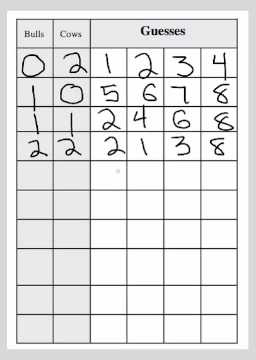
\includegraphics[width=1.0\linewidth,height=0.5\linewidth]{fig080001.png}
  \caption{„Бикове и крави“ \\ https://i.ytimg.com/vi/r\_dw8iV\_52g/hqdefault.jpg}
\label{fig080001}
\end{figure}

Играта „Бикове и крави“ (Фиг. \ref{fig080001}) е от групата игри за разгадаване на шифър. Играе се от двама играчи, с лист и молив, като всеки играч си намисля четири цифрено число (тайна), което не може да започва с цифрата нула. Всеки от играчите се опитва да разгадае числото на противника. Процесът на разгадаване включва споменаването на четири цифрено число, като противникът отговаря с информация за това колко цифри от предположението са на точните си места и колко цифри са на други места. За всяка цифра, която съвпада по позиция с тайното число се докладва по един бик, а за всяка цифра, която не съвпада по позиция се докладва по една крава. Играта приключва, когато един от играчите успее да предположи число, което води до четири бика. 

\section{Оформяне на графичния интерфейс}

Играта не е сложна, но е идеален вариант да се демонстрира компютърен опонент, който използва похвати от теорията за множествата. Разработката на играта започва със създаването на нов проект (Фиг. \ref{fig080002}).

\begin{figure}[H]
  \centering
  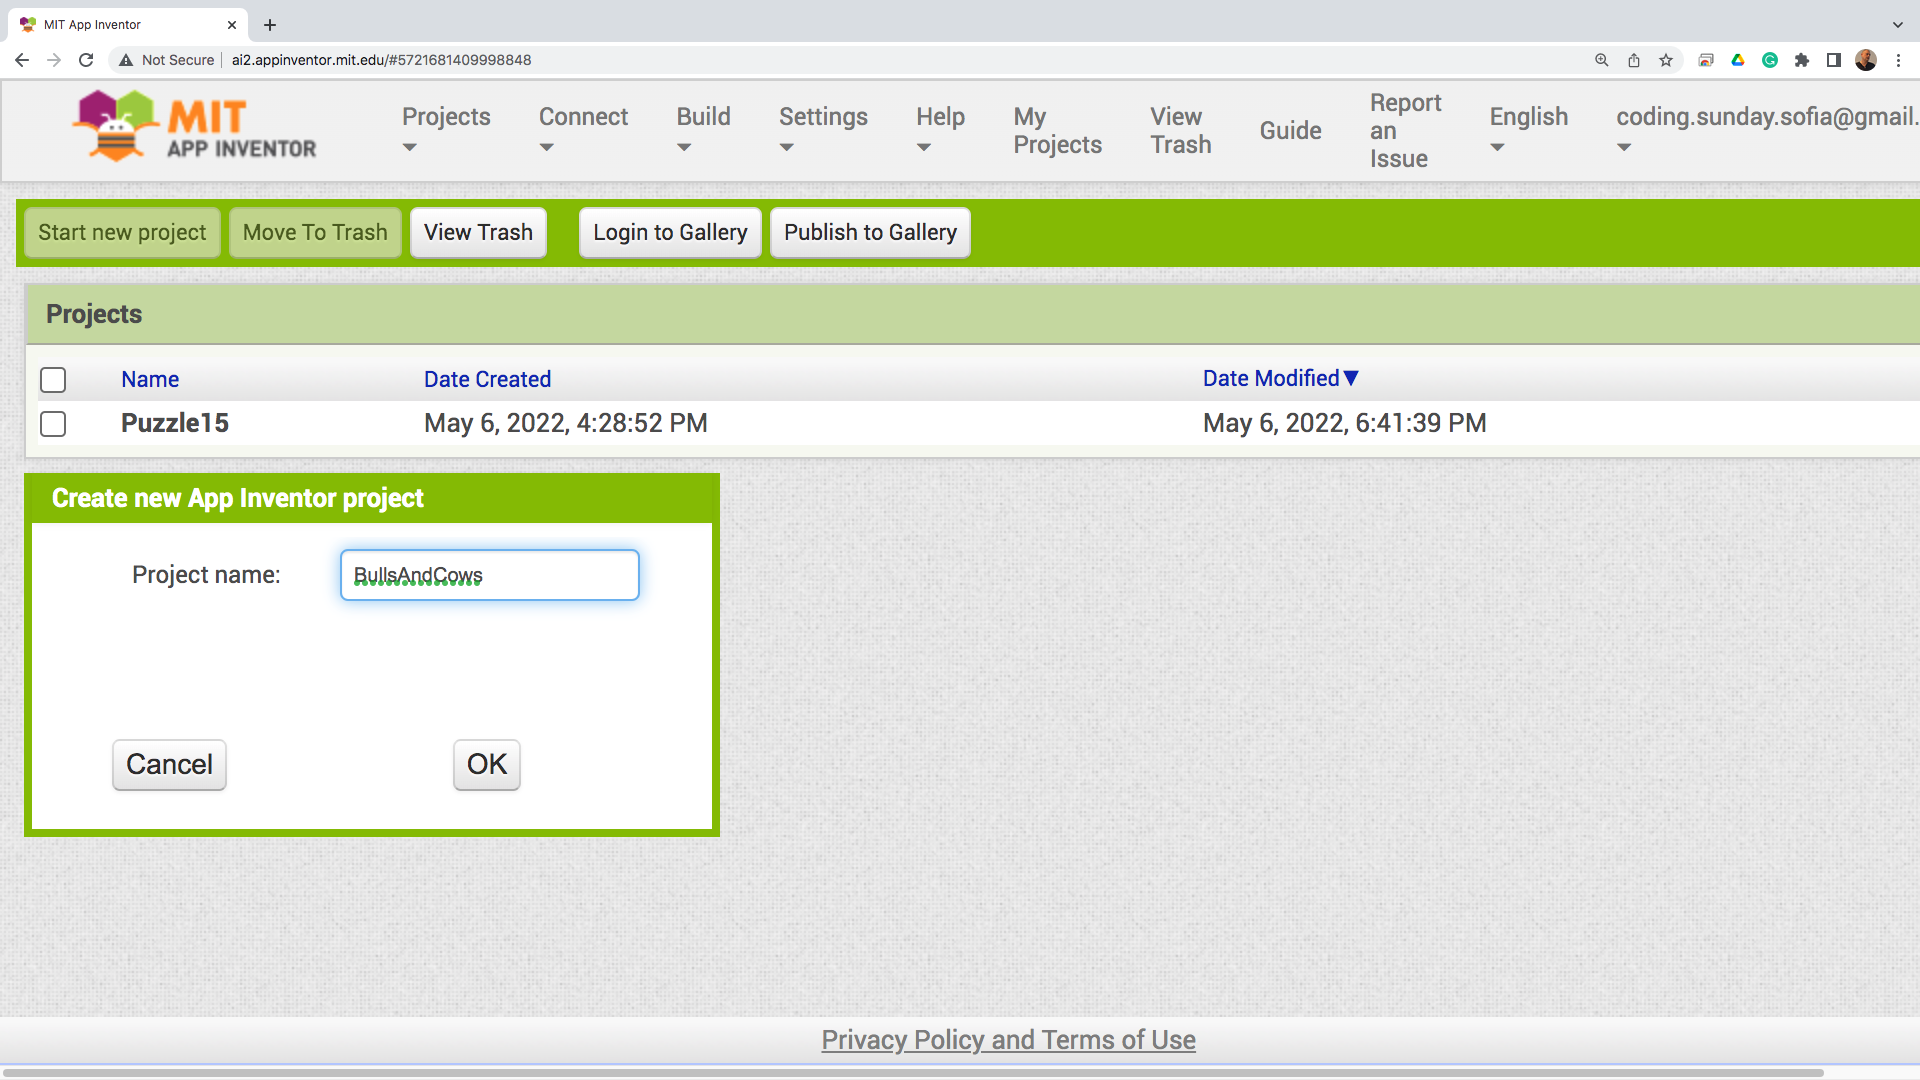
\includegraphics[width=1.0\linewidth,height=0.5\linewidth]{fig080002.png}
  \caption{Създаване на нов проект за „Бикове и крави“}
\label{fig080002}
\end{figure}

Възможни са различни начини за организиране на графичния потребителски интерфейс, но с демонстрационна цел е удачно да се използва най-опростеният вариант. В мениджър за управление на визуалните колони от тип таблица може да се разположат визуални контроли в матрица от 9 колони и 2 реда (Фиг. \ref{fig080003}).

\begin{figure}[H]
  \centering
  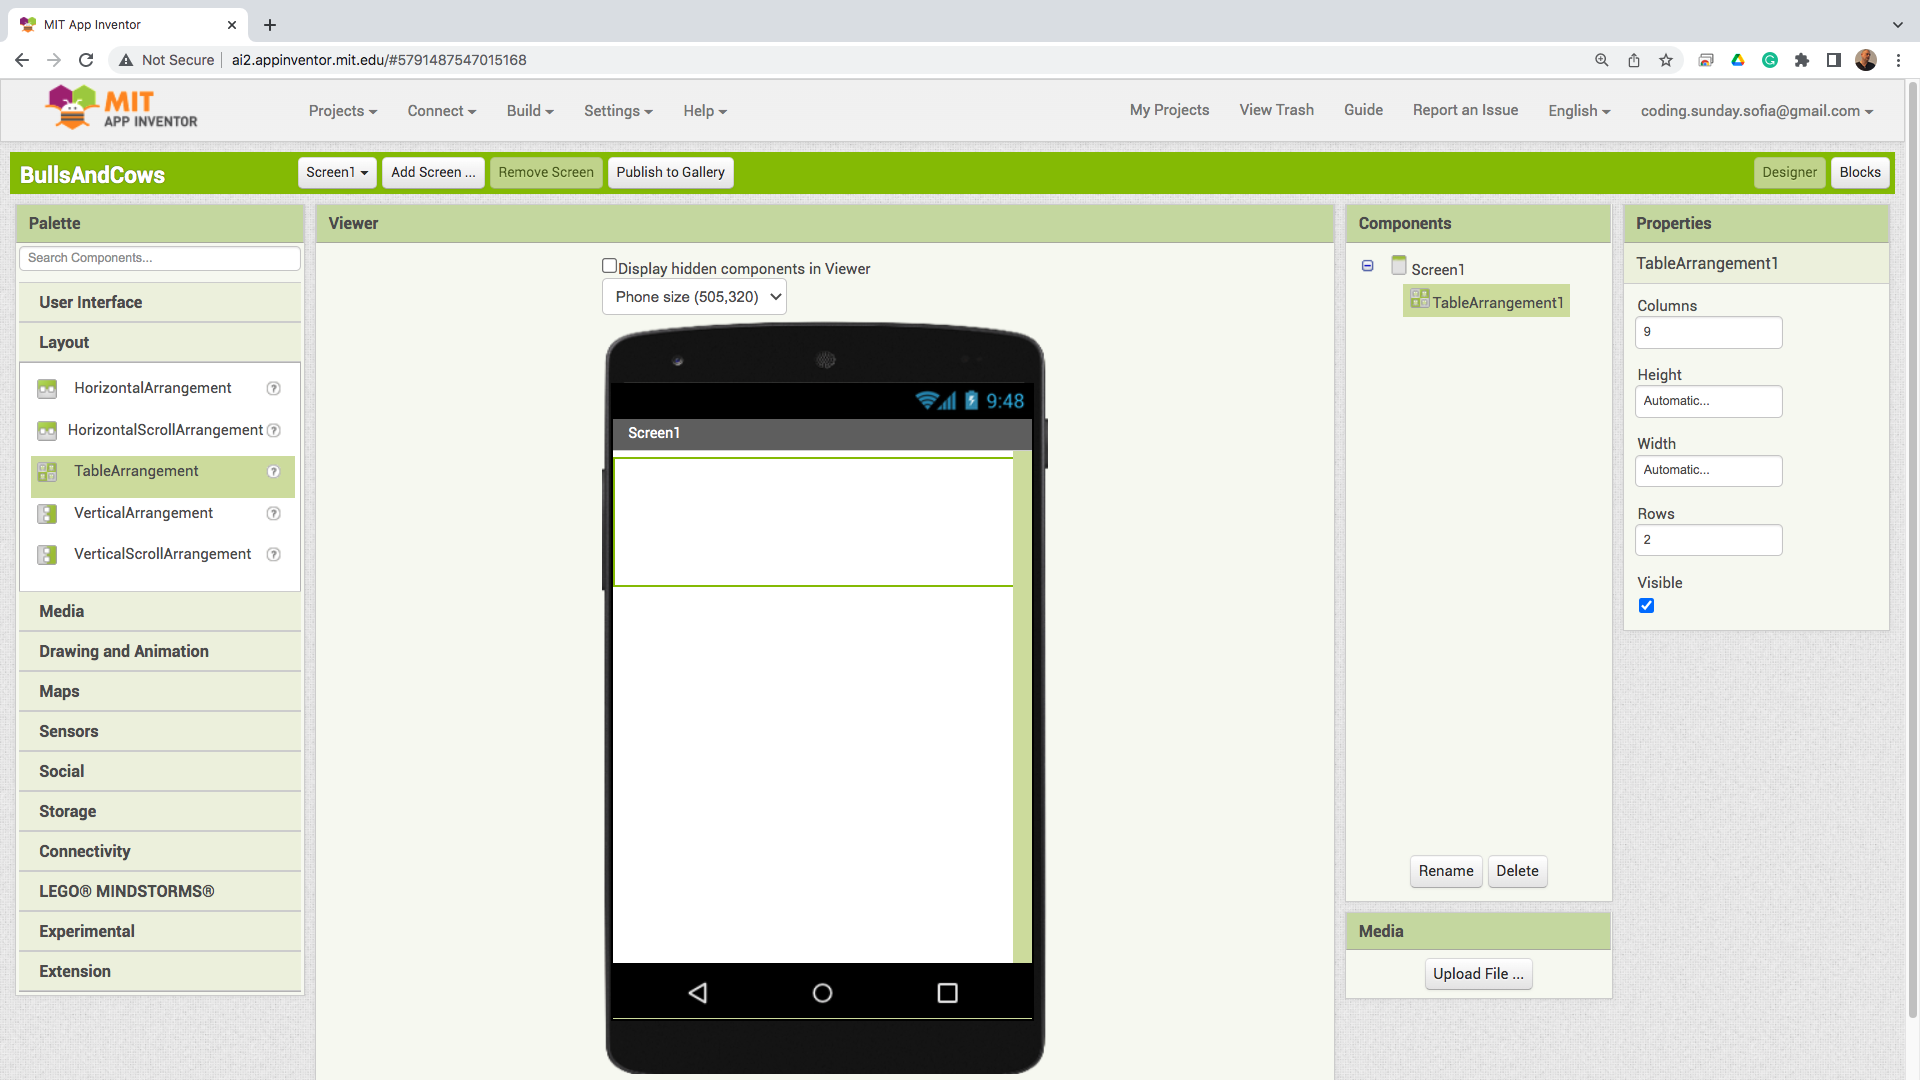
\includegraphics[width=1.0\linewidth,height=0.5\linewidth]{fig080003.png}
  \caption{Мениджър на визуалните компоненти 9x2}
\label{fig080003}
\end{figure}

Тъй като всеки играч прави запитвания за четири цифрени числа, то на първия ред в таблицата, първите четири позиции, се запълват с четири визуални компонента за избор от списък (Фиг. \ref{fig080004}). Тези четири списъчни контроли ще служат за визуализация на четири цифрените числа, предполагани от компютърния опонент. Всеки от компонентите първоначално визуализира символа звезда, а списъка от възможни стойности са цифрите от нула до девет. В първият визуален компонент не би трябвало да е възможно избирането на нулата, но за симетрия нулата е оставена в списъка. 

\begin{figure}[H]
  \centering
  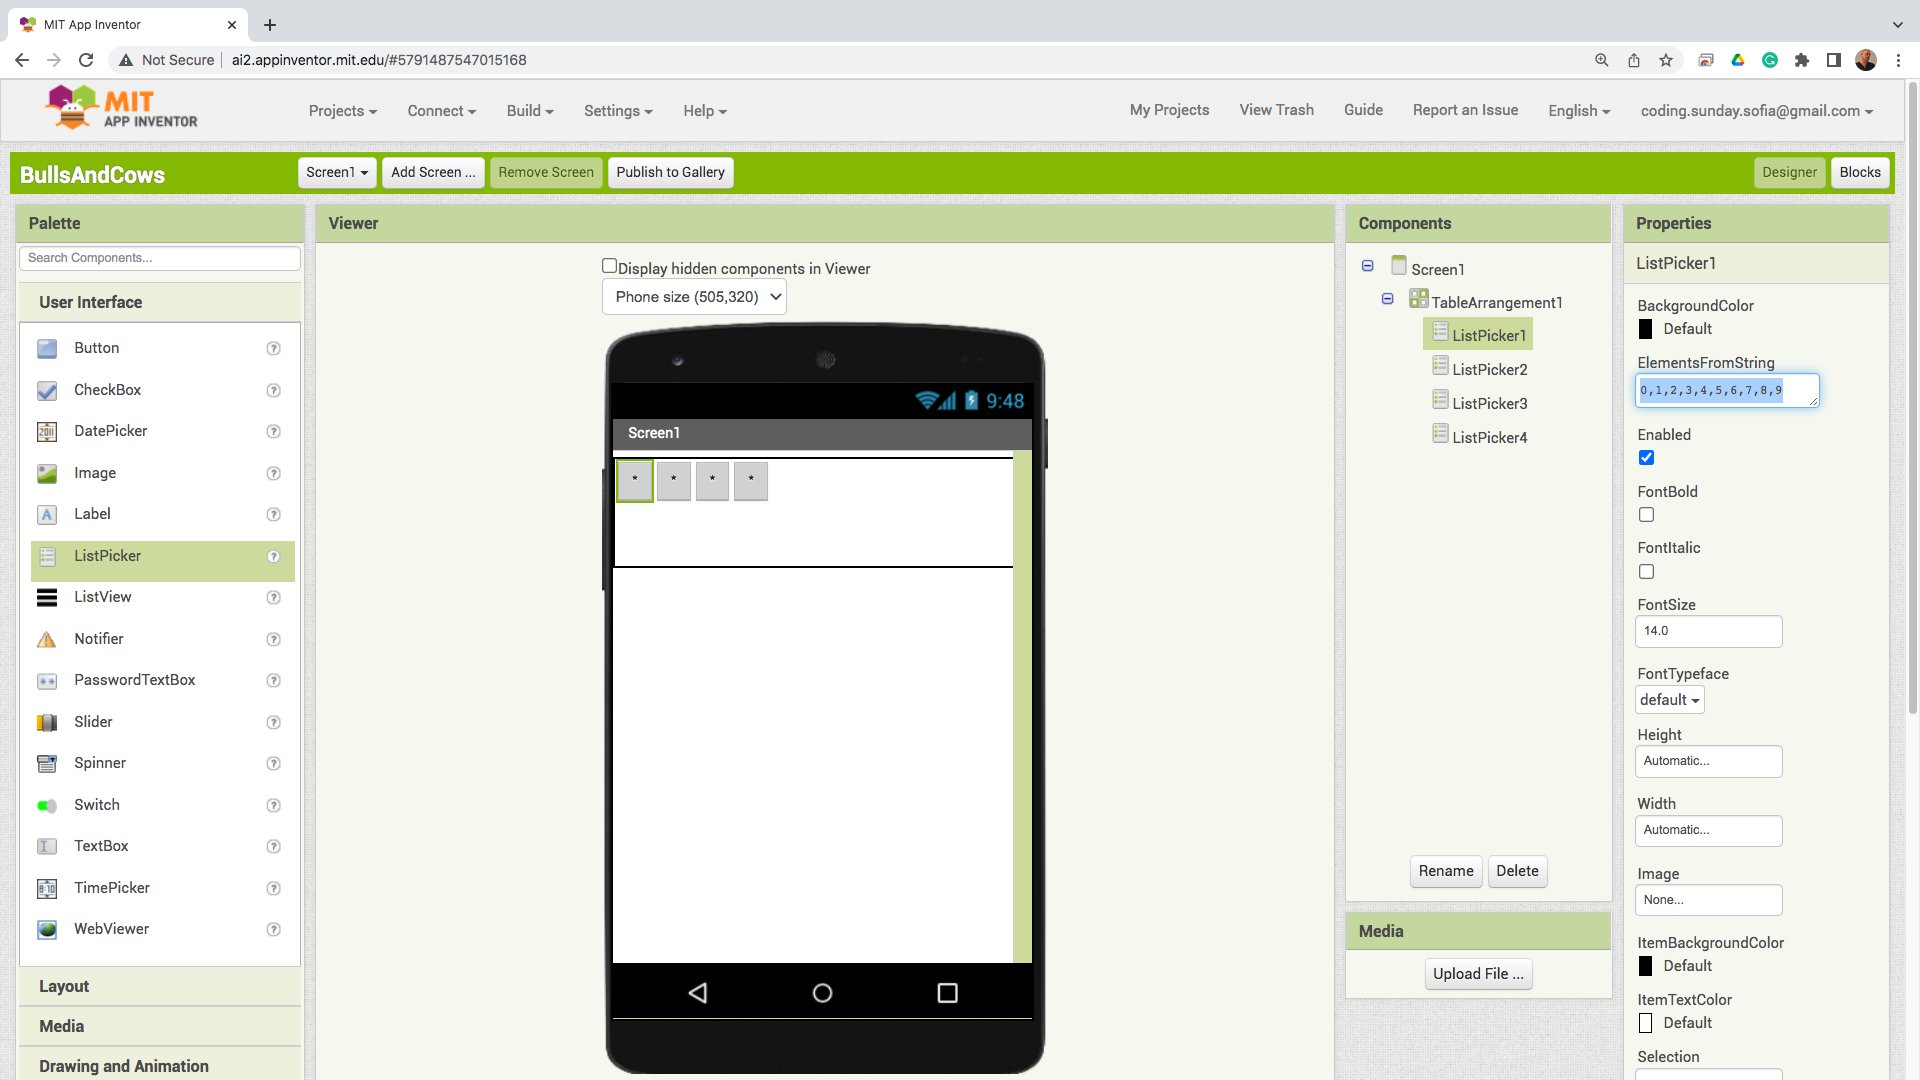
\includegraphics[width=1.0\linewidth,height=0.5\linewidth]{fig080004.png}
  \caption{Визуални контроли за предположенията на компютъра}
\label{fig080004}
\end{figure}

По аналогичен начин се подреждат още четири списъчни контрола (Фиг. \ref{fig080005}), които ще се използват от играча, за да прави предположения кое е тайното число на компютърния опонент. Между двете групи контроли се оставя една празна клетка, която ще бъде използвана за бутон, който да стартира процедурите по разгадаване. 

\begin{figure}[H]
  \centering
  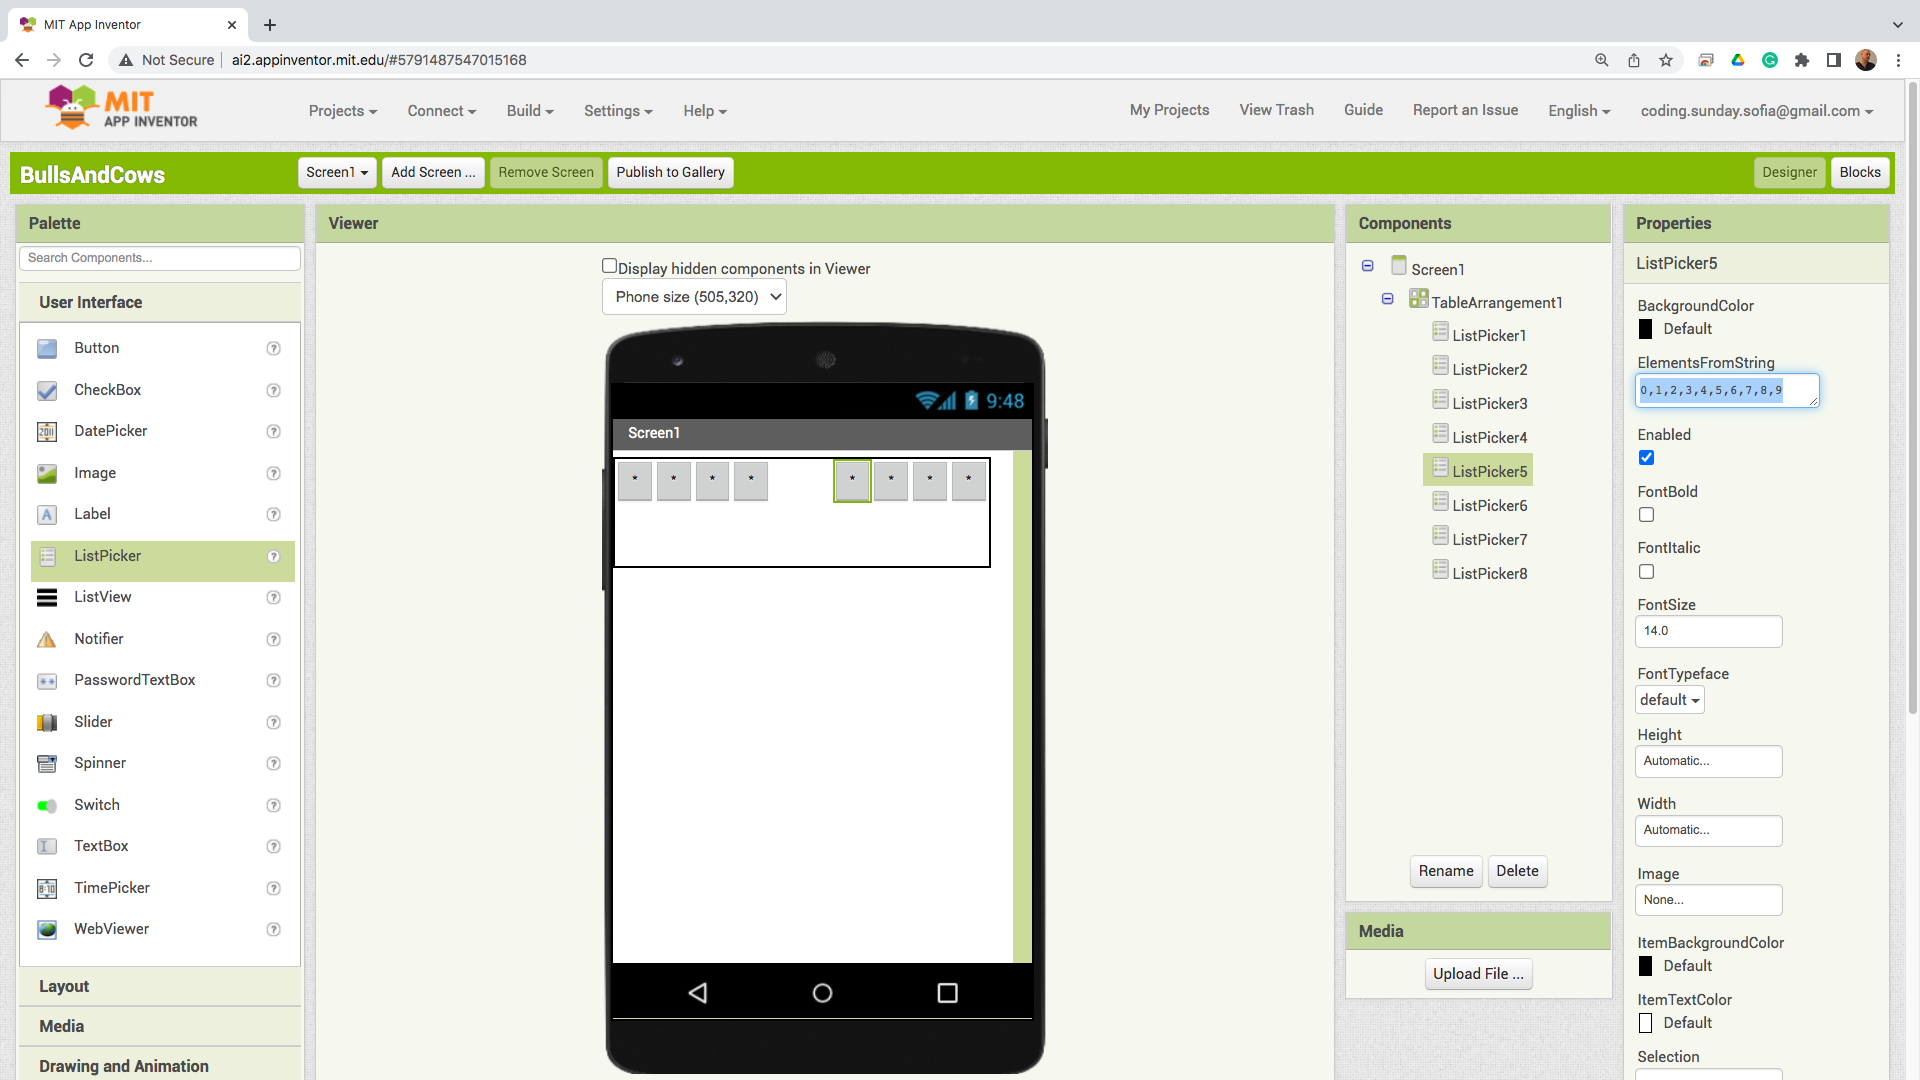
\includegraphics[width=1.0\linewidth,height=0.5\linewidth]{fig080005.png}
  \caption{Визуални контроли за предположенията на човека}
\label{fig080005}
\end{figure}

На втория ред се разполагат още четири списъчни контрола, които ще служат за отбелязване на броя бикове и броя крави (Фиг. \ref{fig080006}). Първите два са за броя бикове и крави, познати от компютърния опонент, а вторите два са за броя бикове и крави, познати от играча. В двойките, левият контрол ще показва биковете, а десният контрол кравите. Възможните опции са от нула до четири, тъй като възможните бикове или крави са от нула, до четири включително.

\begin{figure}[H]
  \centering
  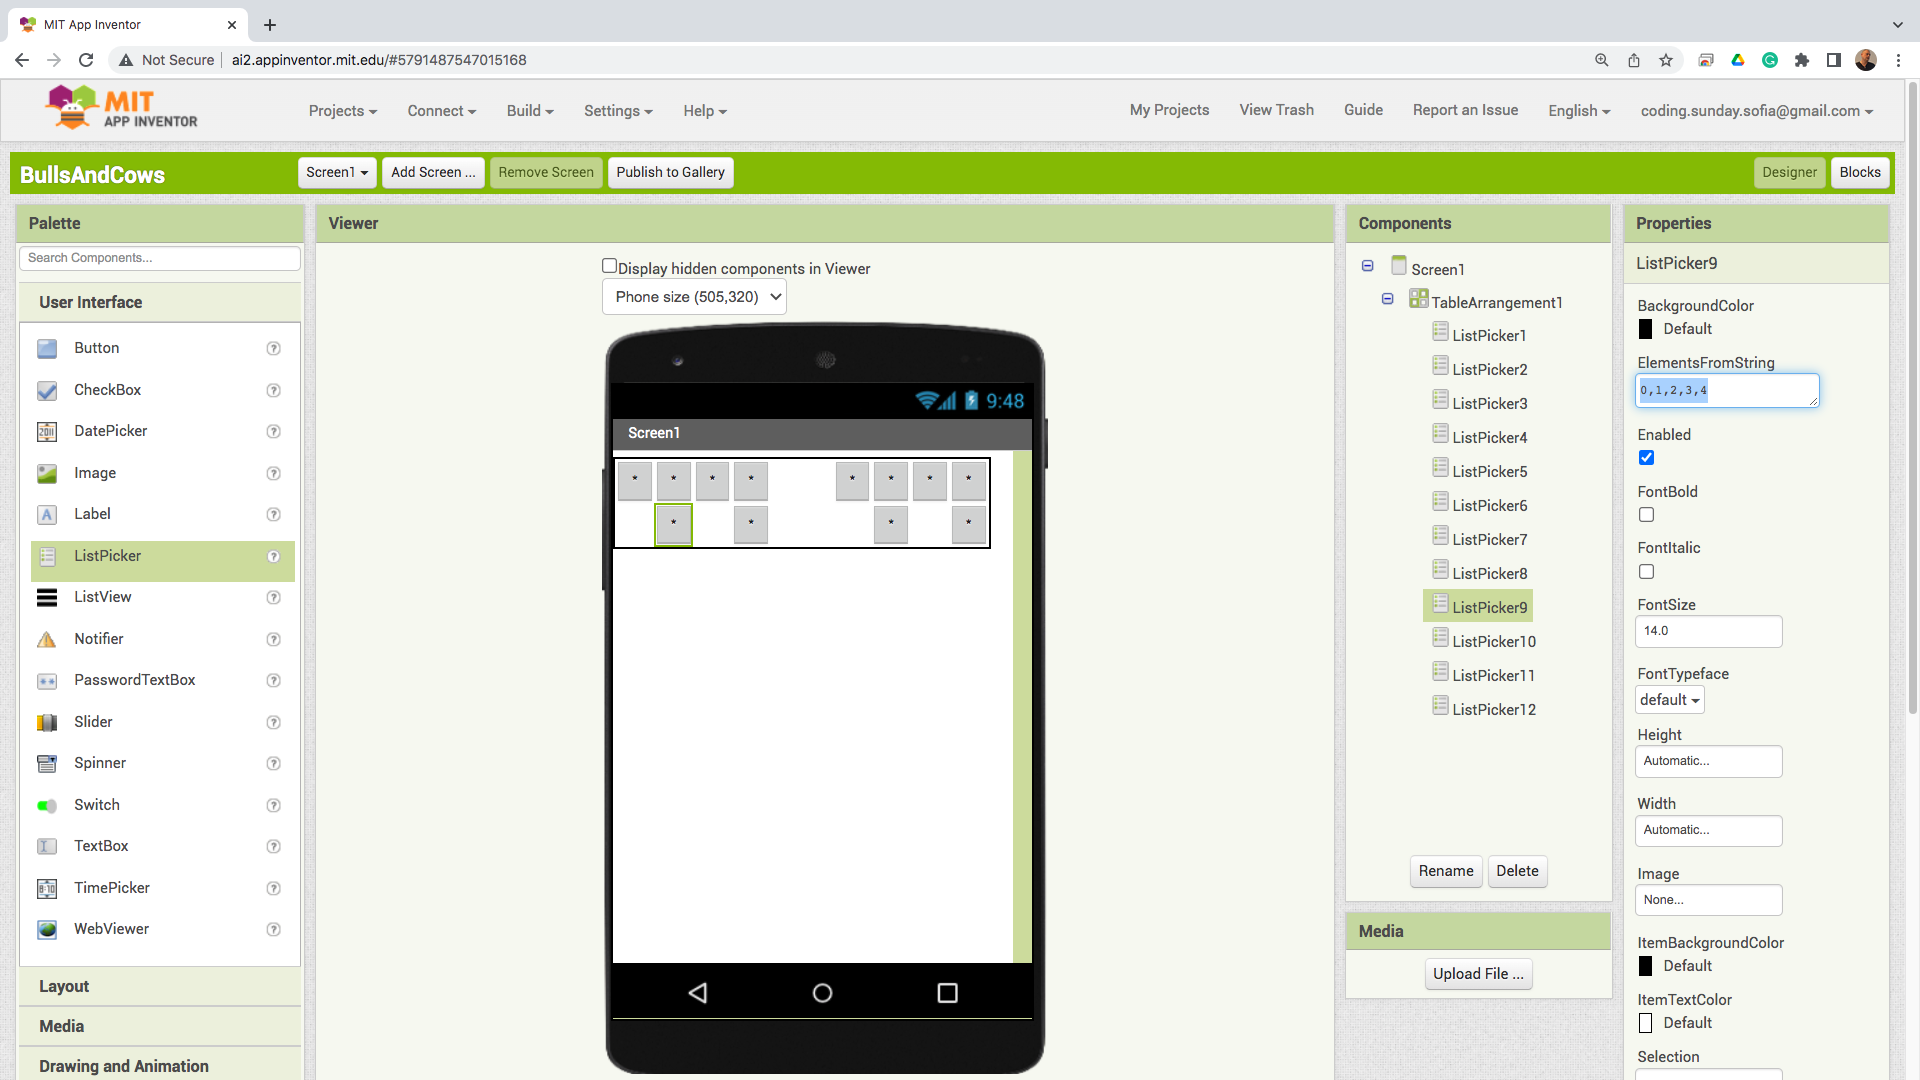
\includegraphics[width=1.0\linewidth,height=0.5\linewidth]{fig080006.png}
  \caption{Визуални контроли за отчитане на биковете и кравите}
\label{fig080006}
\end{figure}

Компонентите за списъчен избор не визуализират в текста си избраната опция автоматично. Поради тази причина е нужно да се прихване събитието за направен избор и избраната опция да се впише в текстовото поле на визуалния компонент. За тази цел се прихваща общо събитие, генерирано от всички списъчни компоненти на екрана (Фиг. \ref{fig080007}).

\begin{figure}[H]
  \centering
  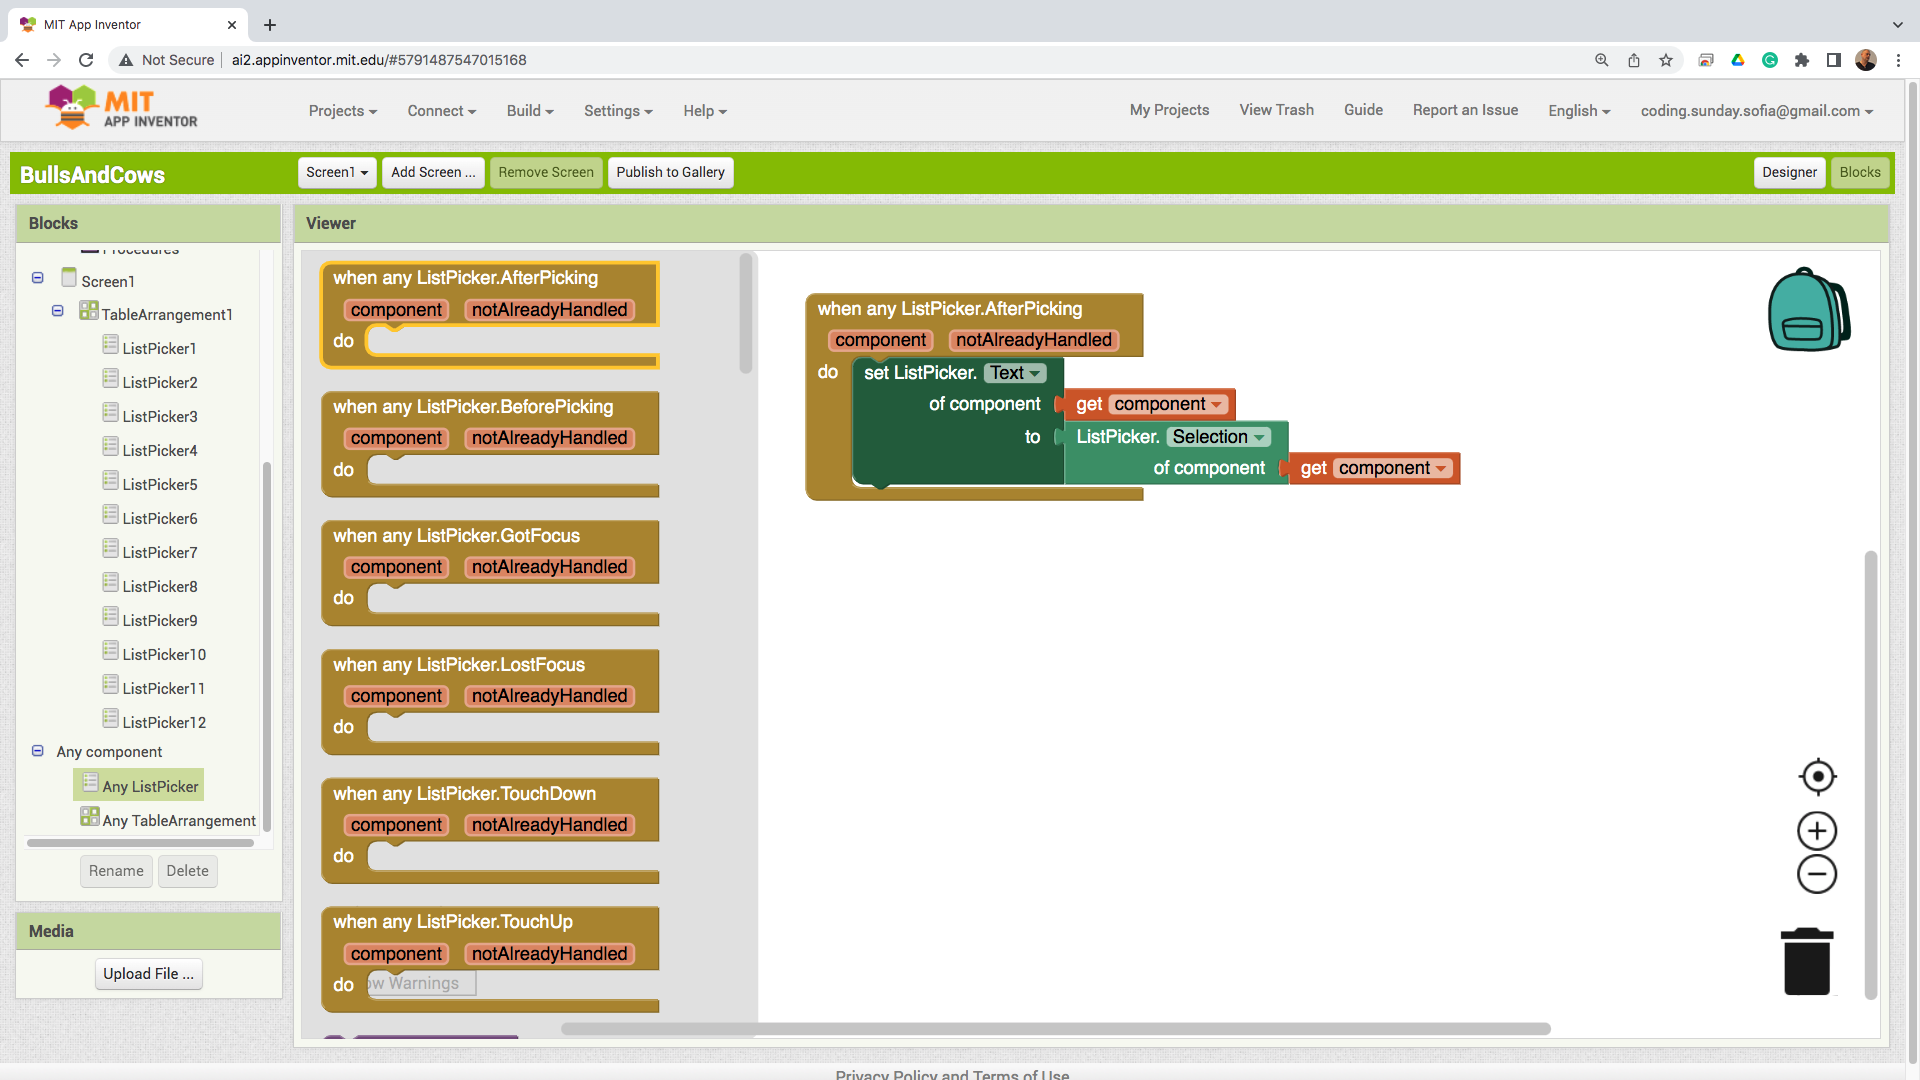
\includegraphics[width=1.0\linewidth,height=0.5\linewidth]{fig080007.png}
  \caption{Визуализация на избраната опция}
\label{fig080007}
\end{figure}

Пред клетките за отчитане на броя бикове и броя крави е разумно да се поставят етикети (Фиг. \ref{fig080008}). Латинската буква B се ползва за биковете, а латинската буква C за броя на кравите. 

\begin{figure}[H]
  \centering
  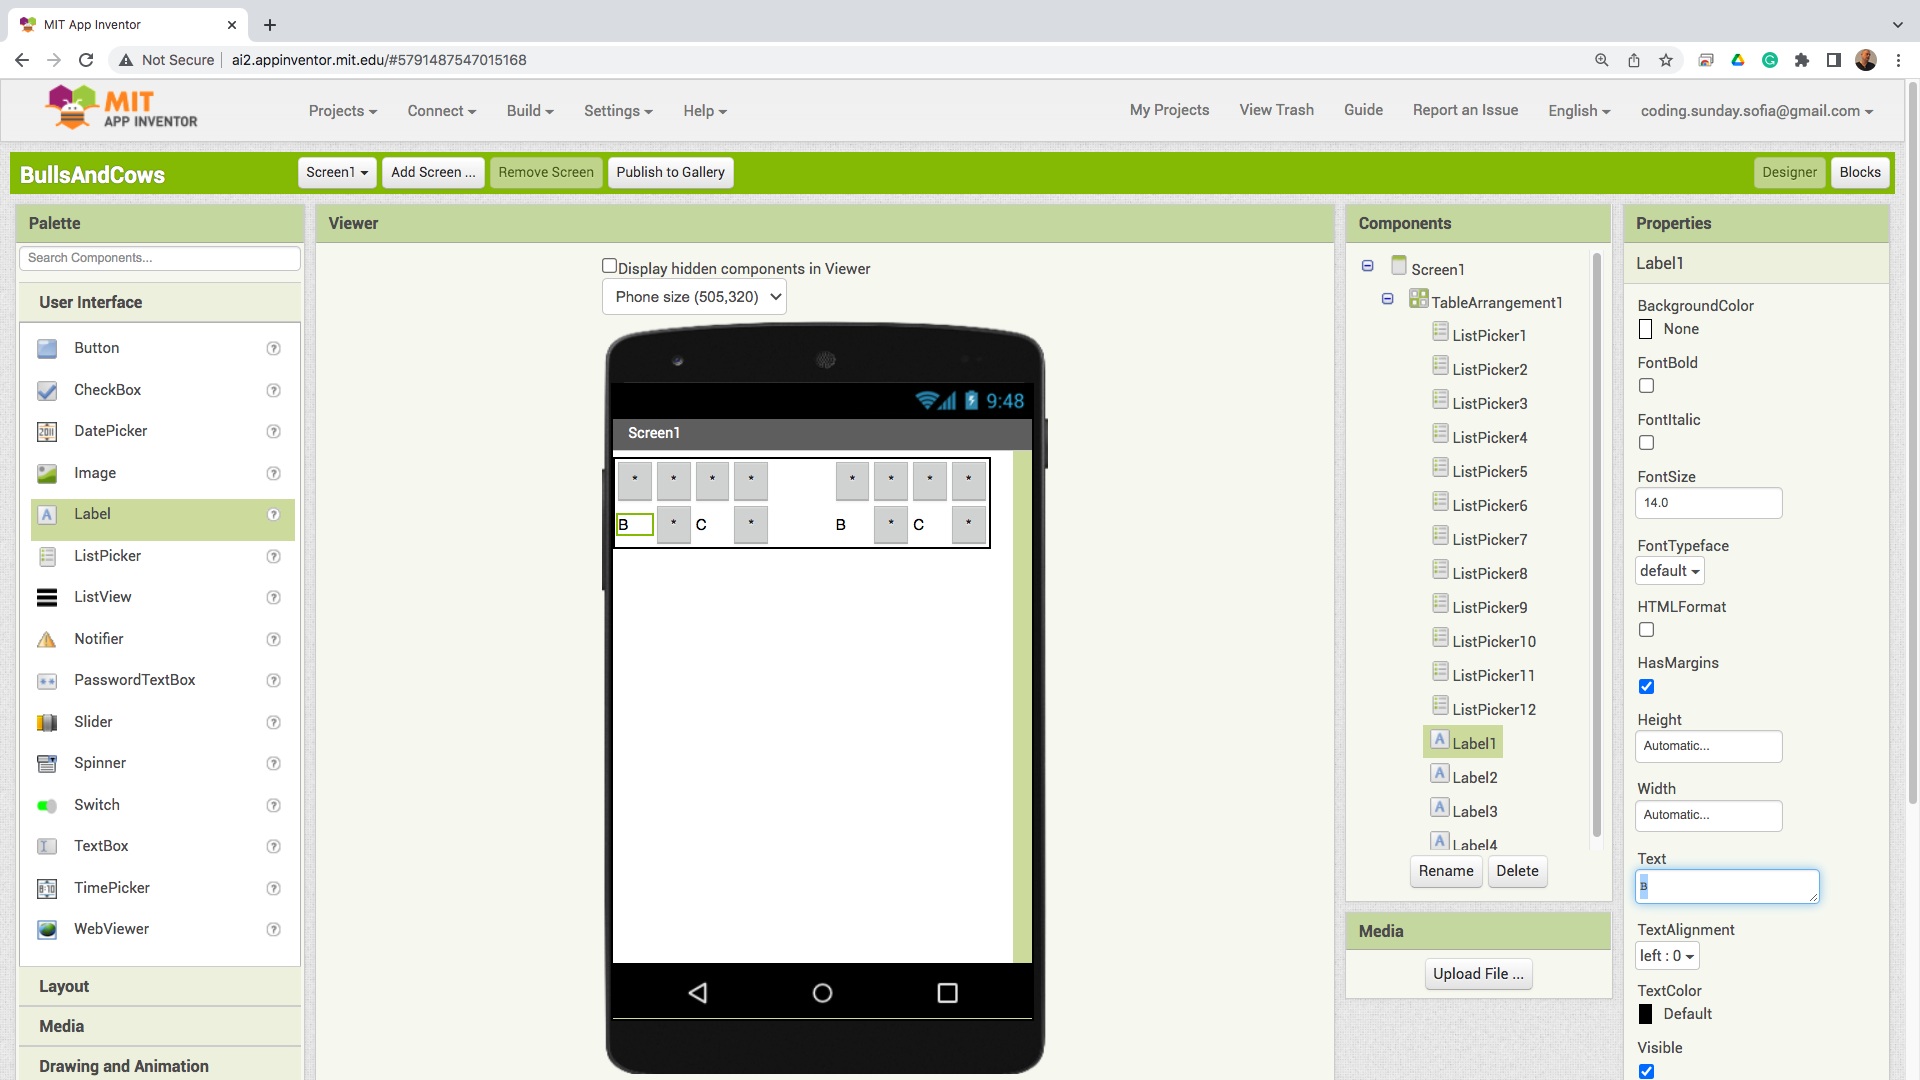
\includegraphics[width=1.0\linewidth,height=0.5\linewidth]{fig080008.png}
  \caption{Етикети пред контролите за отчитане на биковете и кравите}
\label{fig080008}
\end{figure}

Потребителският интерфейс завършва с два бутона (Фиг. \ref{fig080009}). Първият активизира компютърния опонент да познае числото на играча, а втория активизира компютърния опонент да съобщи броя уцелени от човека бикове и крави.

\begin{figure}[H]
  \centering
  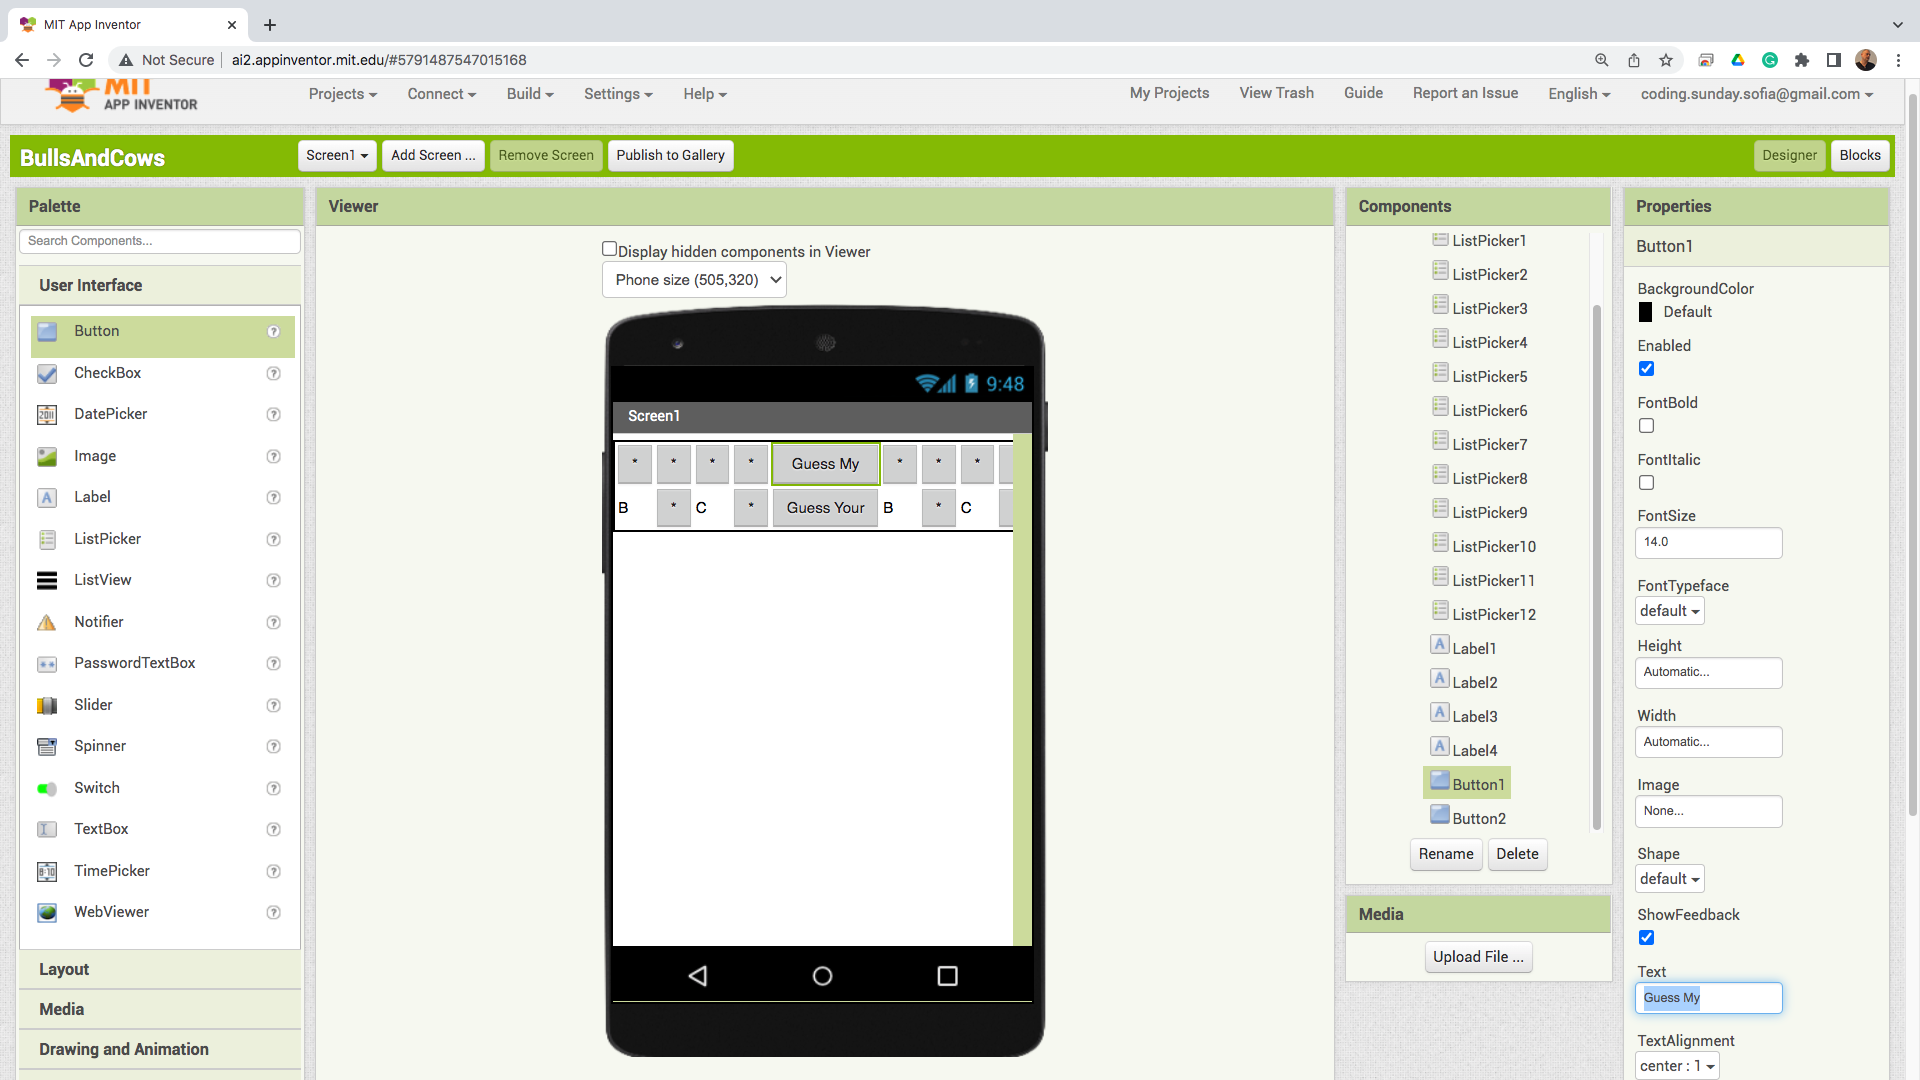
\includegraphics[width=1.0\linewidth,height=0.5\linewidth]{fig080009.png}
  \caption{Бутони за активизиране на процеса по разгадаване}
\label{fig080009}
\end{figure}

\section{Използване на структури от данни}

За нуждите на компютърния опонент и според теорията на множествата, важно е да се създаде списъчна структура (Фиг. \ref{fig080010}), която да съдържа всички възможни комбинации на четири цифрени числа, цифрите на които не се повтарят и не започват с нула. При всеки отговор на човека, от списъка се изключват всички комбинации, които не отговарят на условията за установени бикове и крави.

\begin{figure}[H]
  \centering
  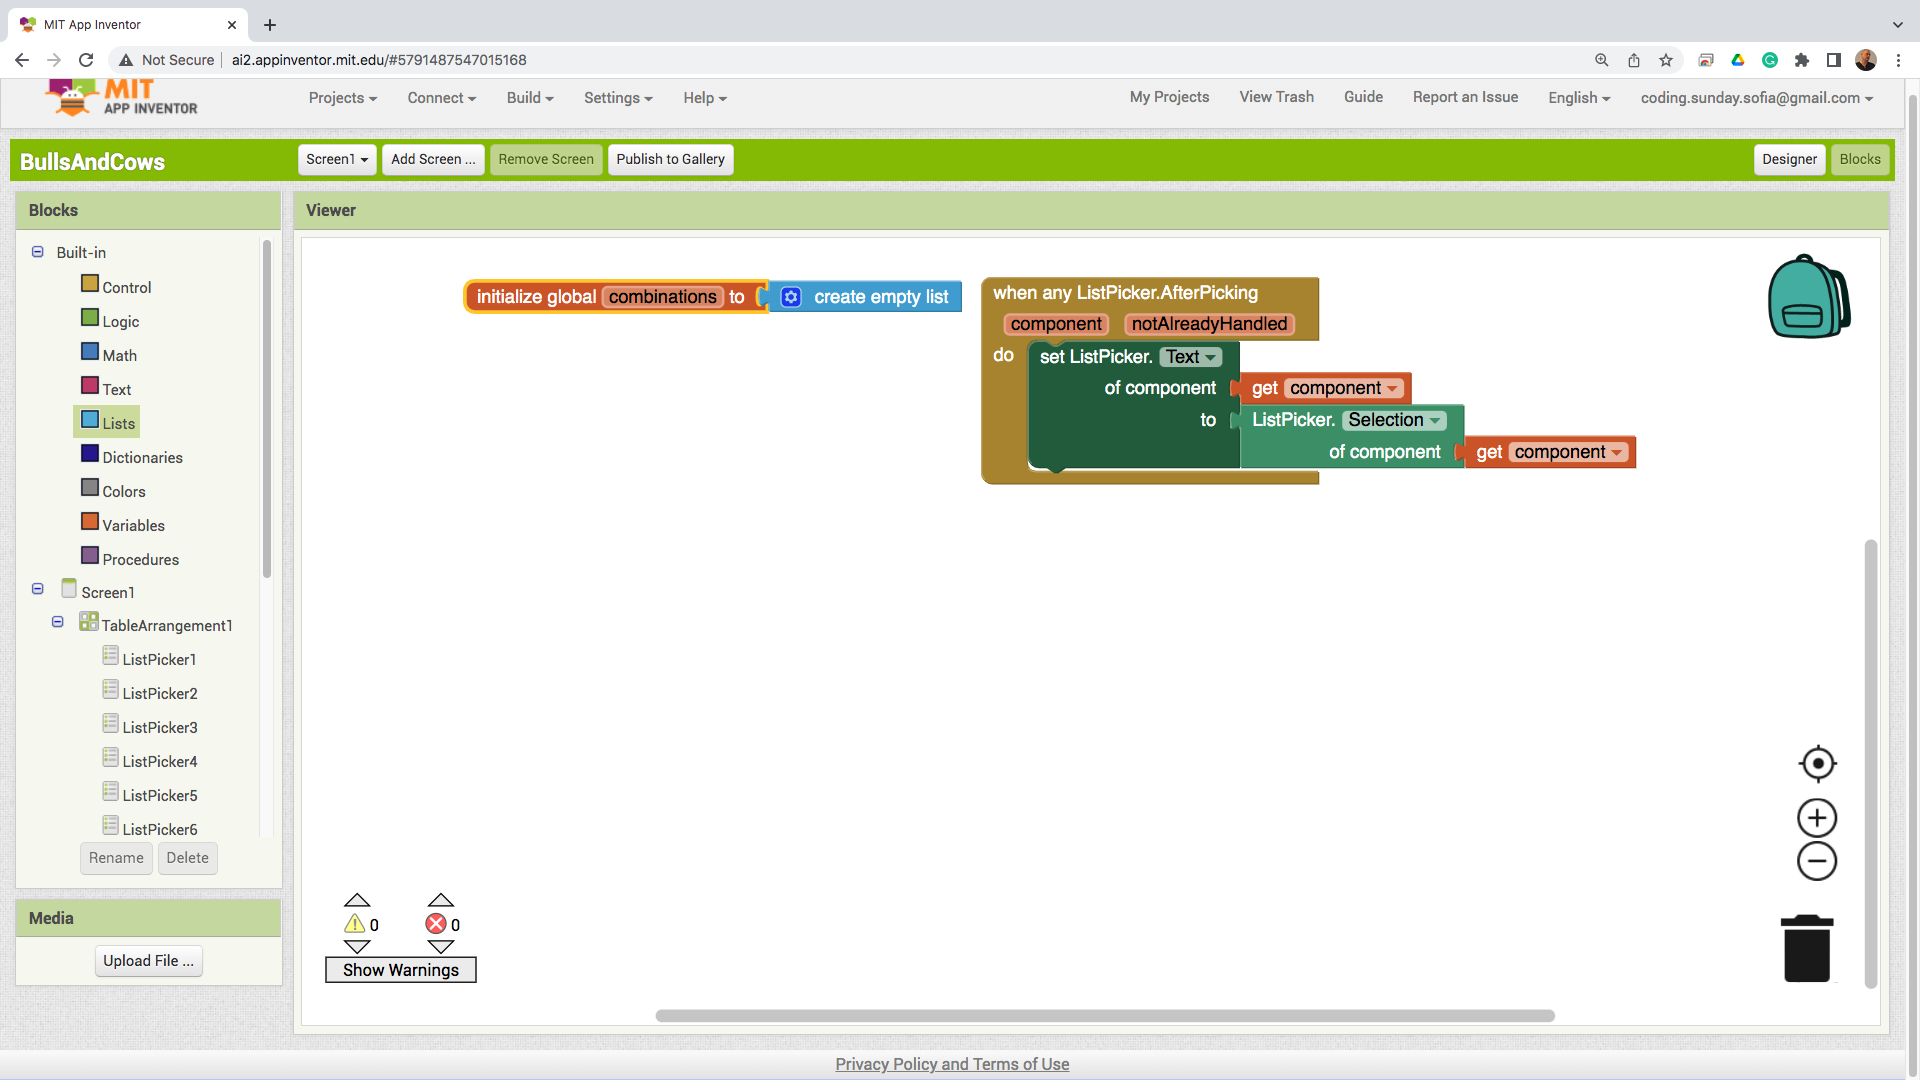
\includegraphics[width=1.0\linewidth,height=0.5\linewidth]{fig080010.png}
  \caption{Списък на комбинациите}
\label{fig080010}
\end{figure}

Числата са четири цифрени, така че списъкът с комбинациите може да се запълни с помощта на четири цикъла (Фиг. \ref{fig080011}). Първият се върти от едно до девет, тъй като нулата не може да участва, като първа цифра. Другите три цикъла се въртят от нула до девет. За броячи на циклите се избират латинските букви a, b, c и d. Всеки от броячите ще участва във формирането на четири цифрено число.

\begin{figure}[H]
  \centering
  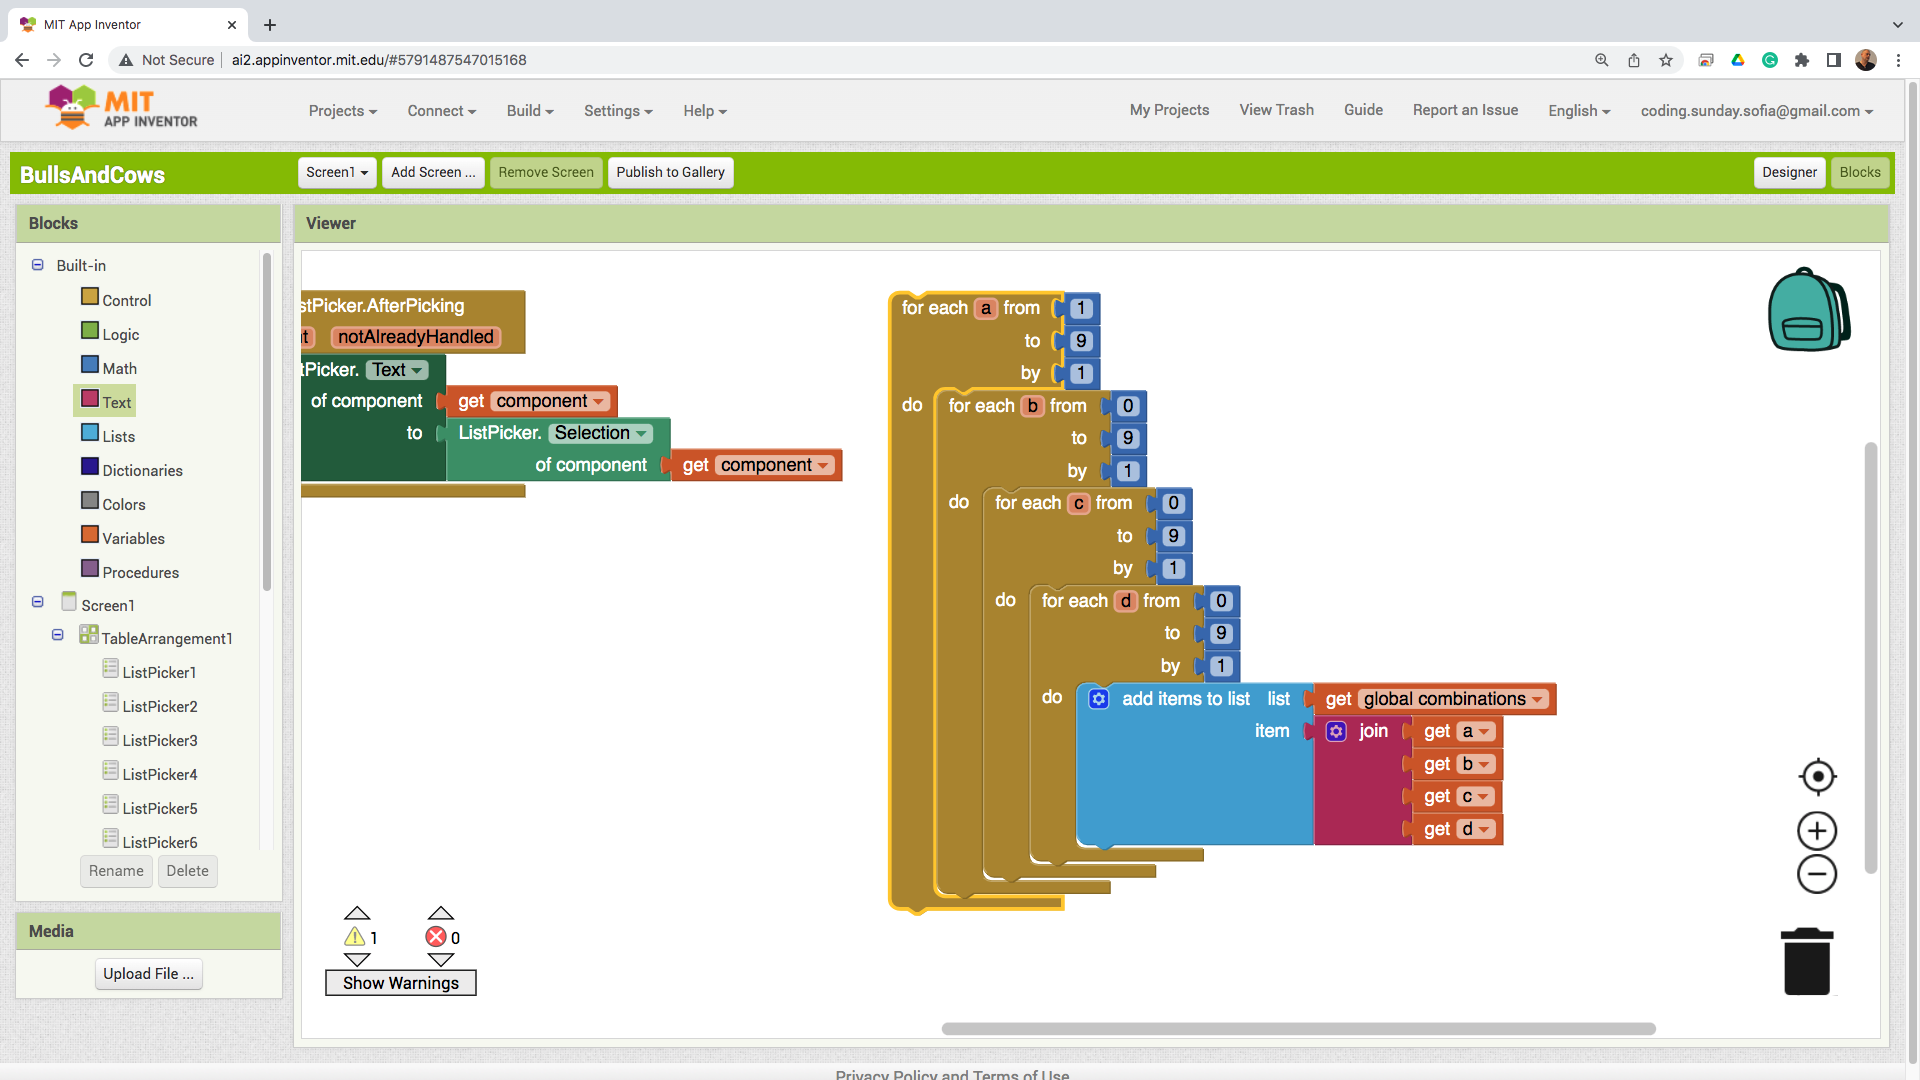
\includegraphics[width=1.0\linewidth,height=0.5\linewidth]{fig080011.png}
  \caption{Цикли за генериране на комбинациите}
\label{fig080011}
\end{figure}

За да се избегне повторение на цифрите е нужно да се направят серия проверки (Фиг. \ref{fig080012}). За първия цикъл проверка няма да се прави, но вторият цикъл се завърта само, ако броячът b се различава от брояча a. Третият цикъл се завърта само, ако броячът c се различава от брояча a и броячът c се различава от брояча b. Четвъртият цикъл се завърта само, ако броячът d се различава от брояча a, различава се от брояча b и се различава от брояча c. 

\begin{figure}[H]
  \centering
  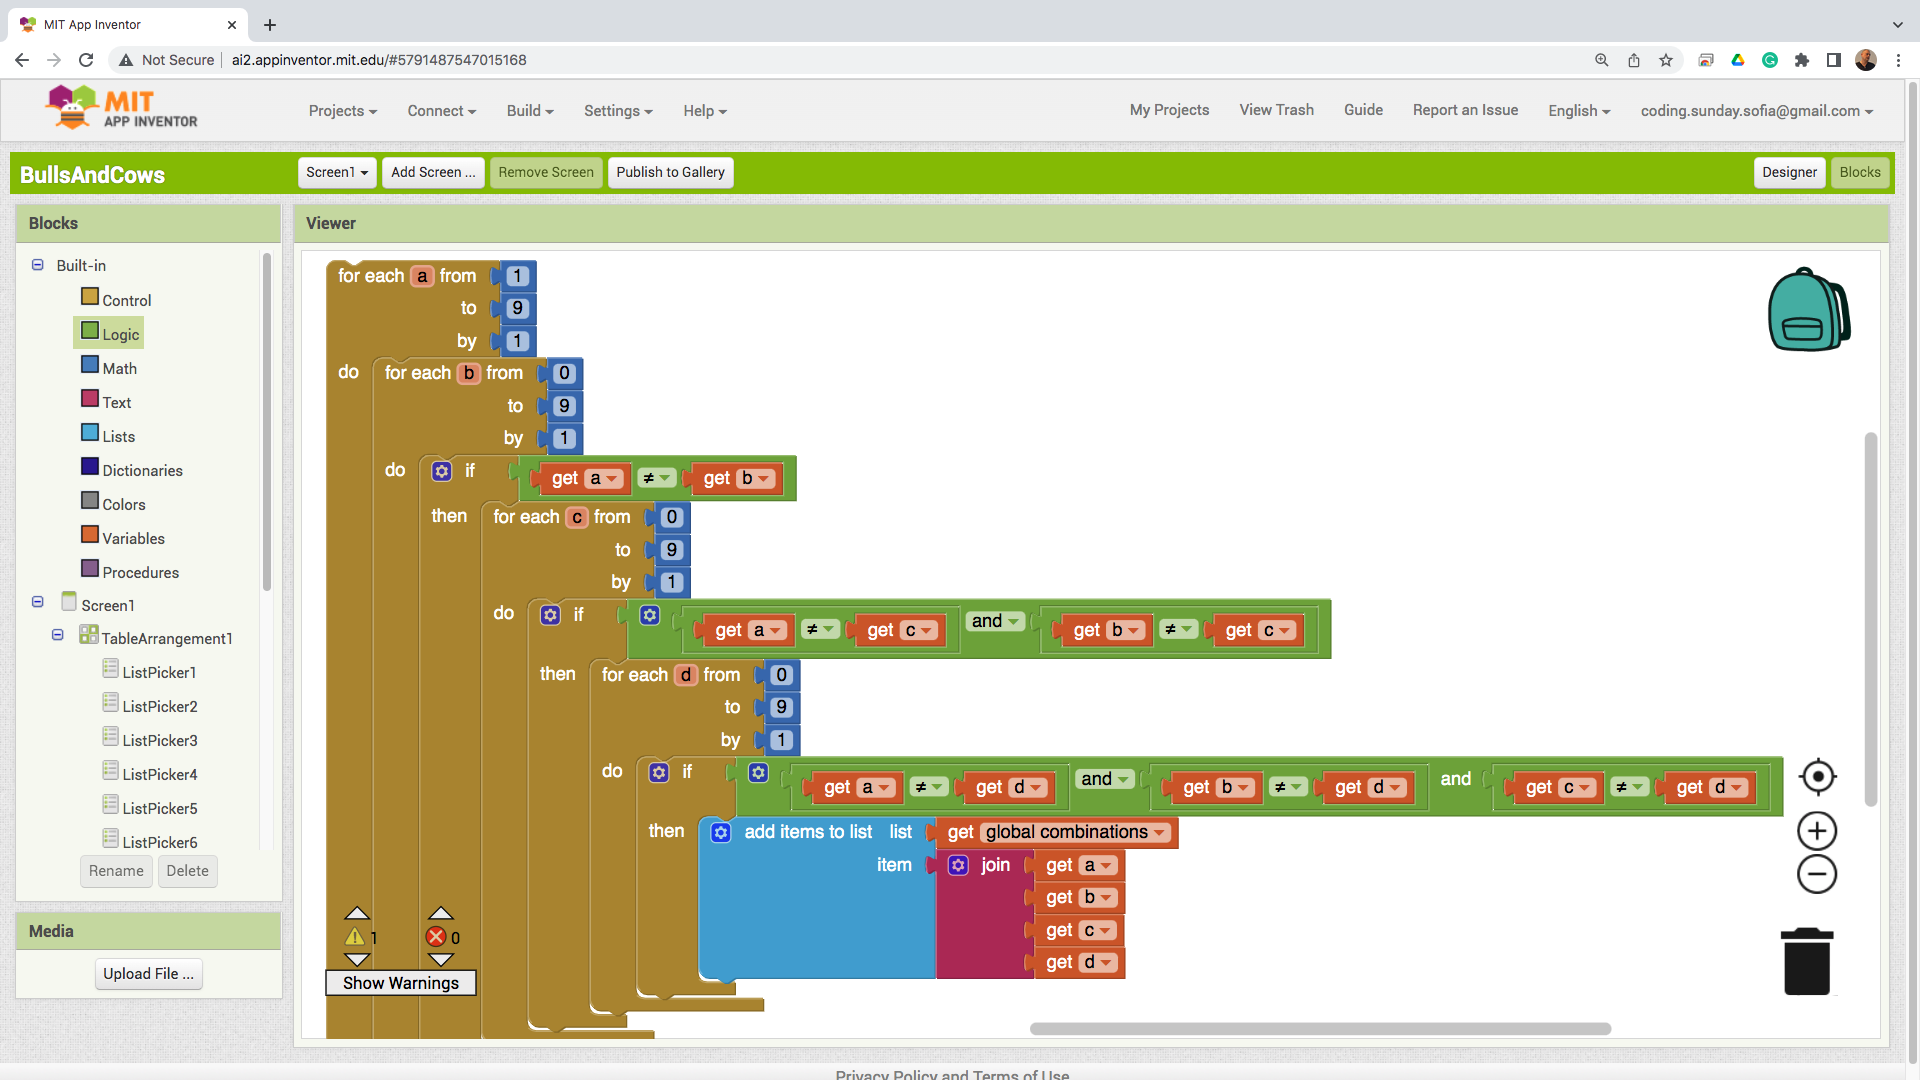
\includegraphics[width=1.0\linewidth,height=0.5\linewidth]{fig080012.png}
  \caption{Проверки за избягване на дублиращи се цифри}
\label{fig080012}
\end{figure}

Две глобални променливи спомагат за съхраняването на тайните числа за компютърния опонент и опонентът човек (Фиг. \ref{fig080013}). Още две глобални променливи пък помагат за обработка на предположението от компютърния опонент и предположението на човека. И четирите променливи, първоначално са служебно инициализирани с нули.

\begin{figure}[H]
  \centering
  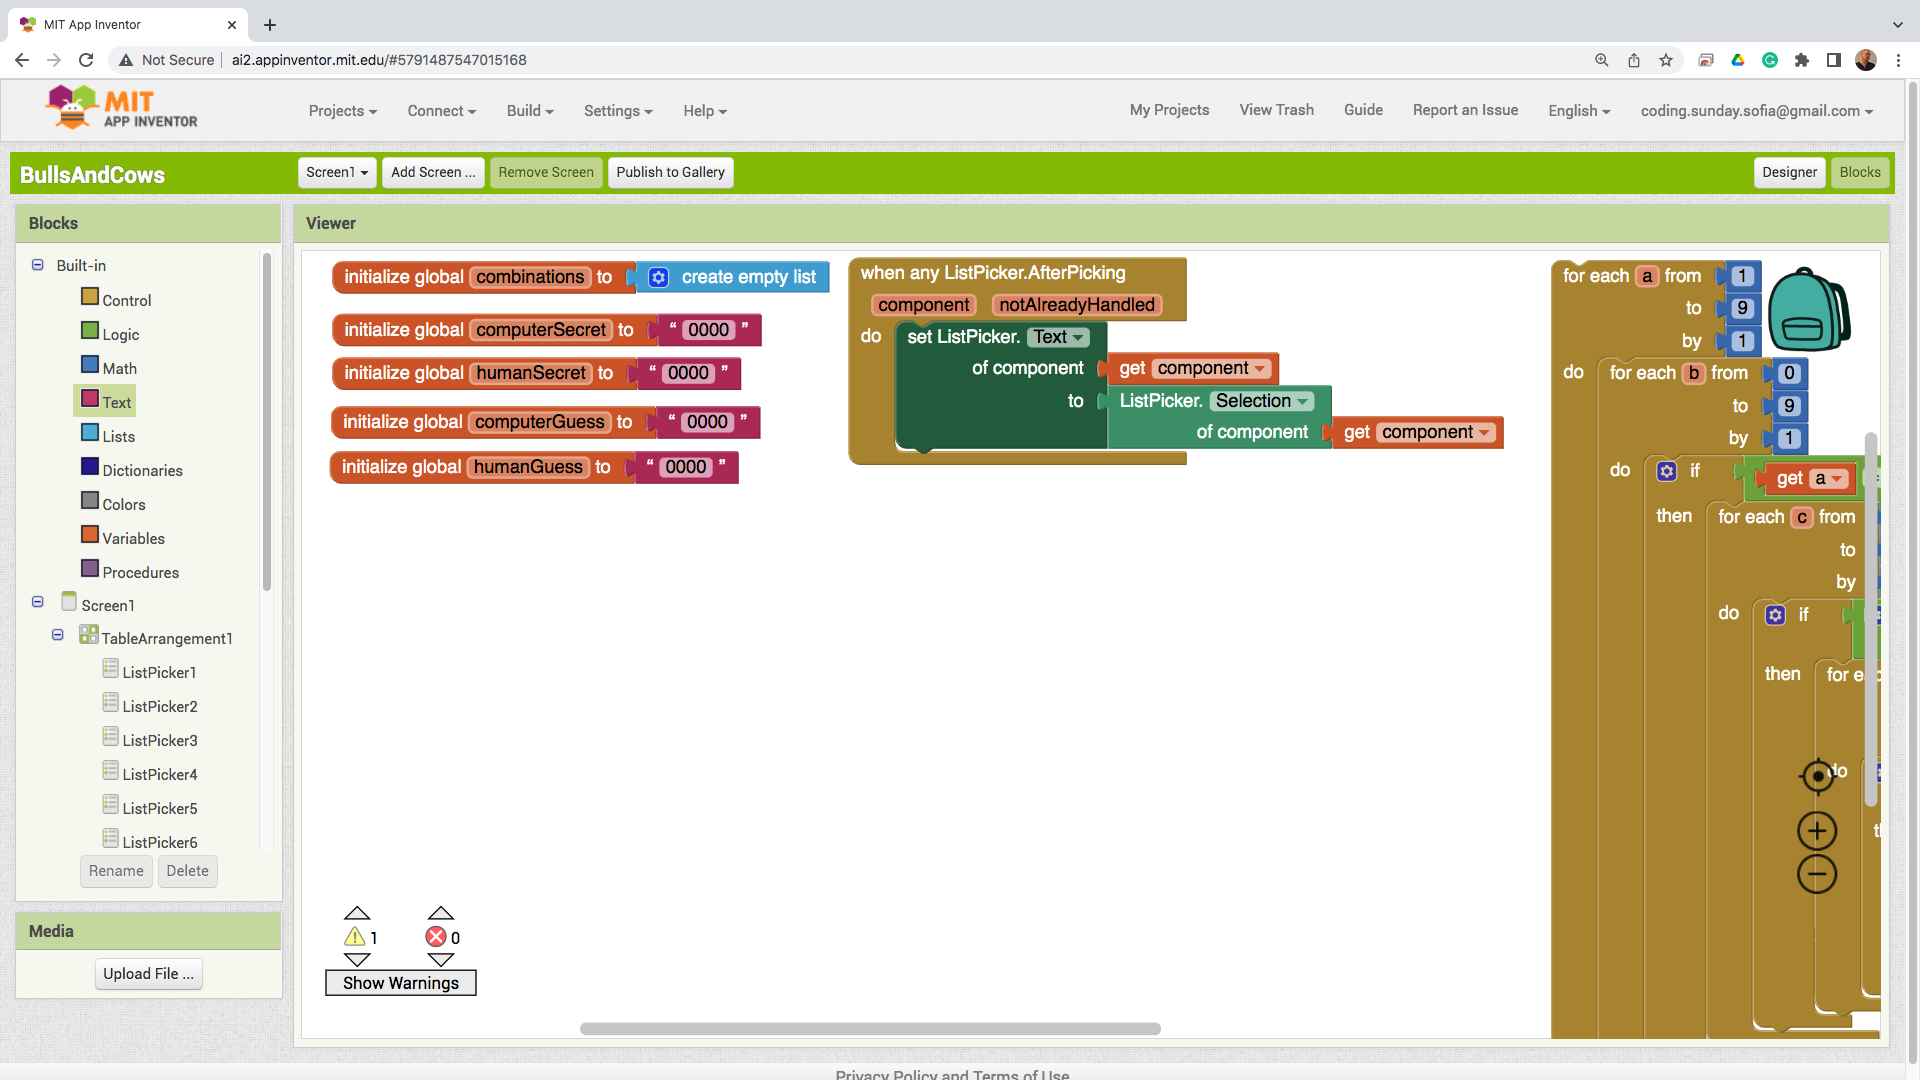
\includegraphics[width=1.0\linewidth,height=0.5\linewidth]{fig080013.png}
  \caption{Помощни променливи за тайните числа на играчите}
\label{fig080013}
\end{figure}

\section{Алгоритми за манипулации в играта}

Циклите за инициализация на списъка с комбинации и последващия избор на една от тях, като тайно число на компютърния опонент, трябва да се случат в събитие маркиращо инициализацията на работния екран (Фиг. \ref{fig080014}).

\begin{figure}[H]
  \centering
  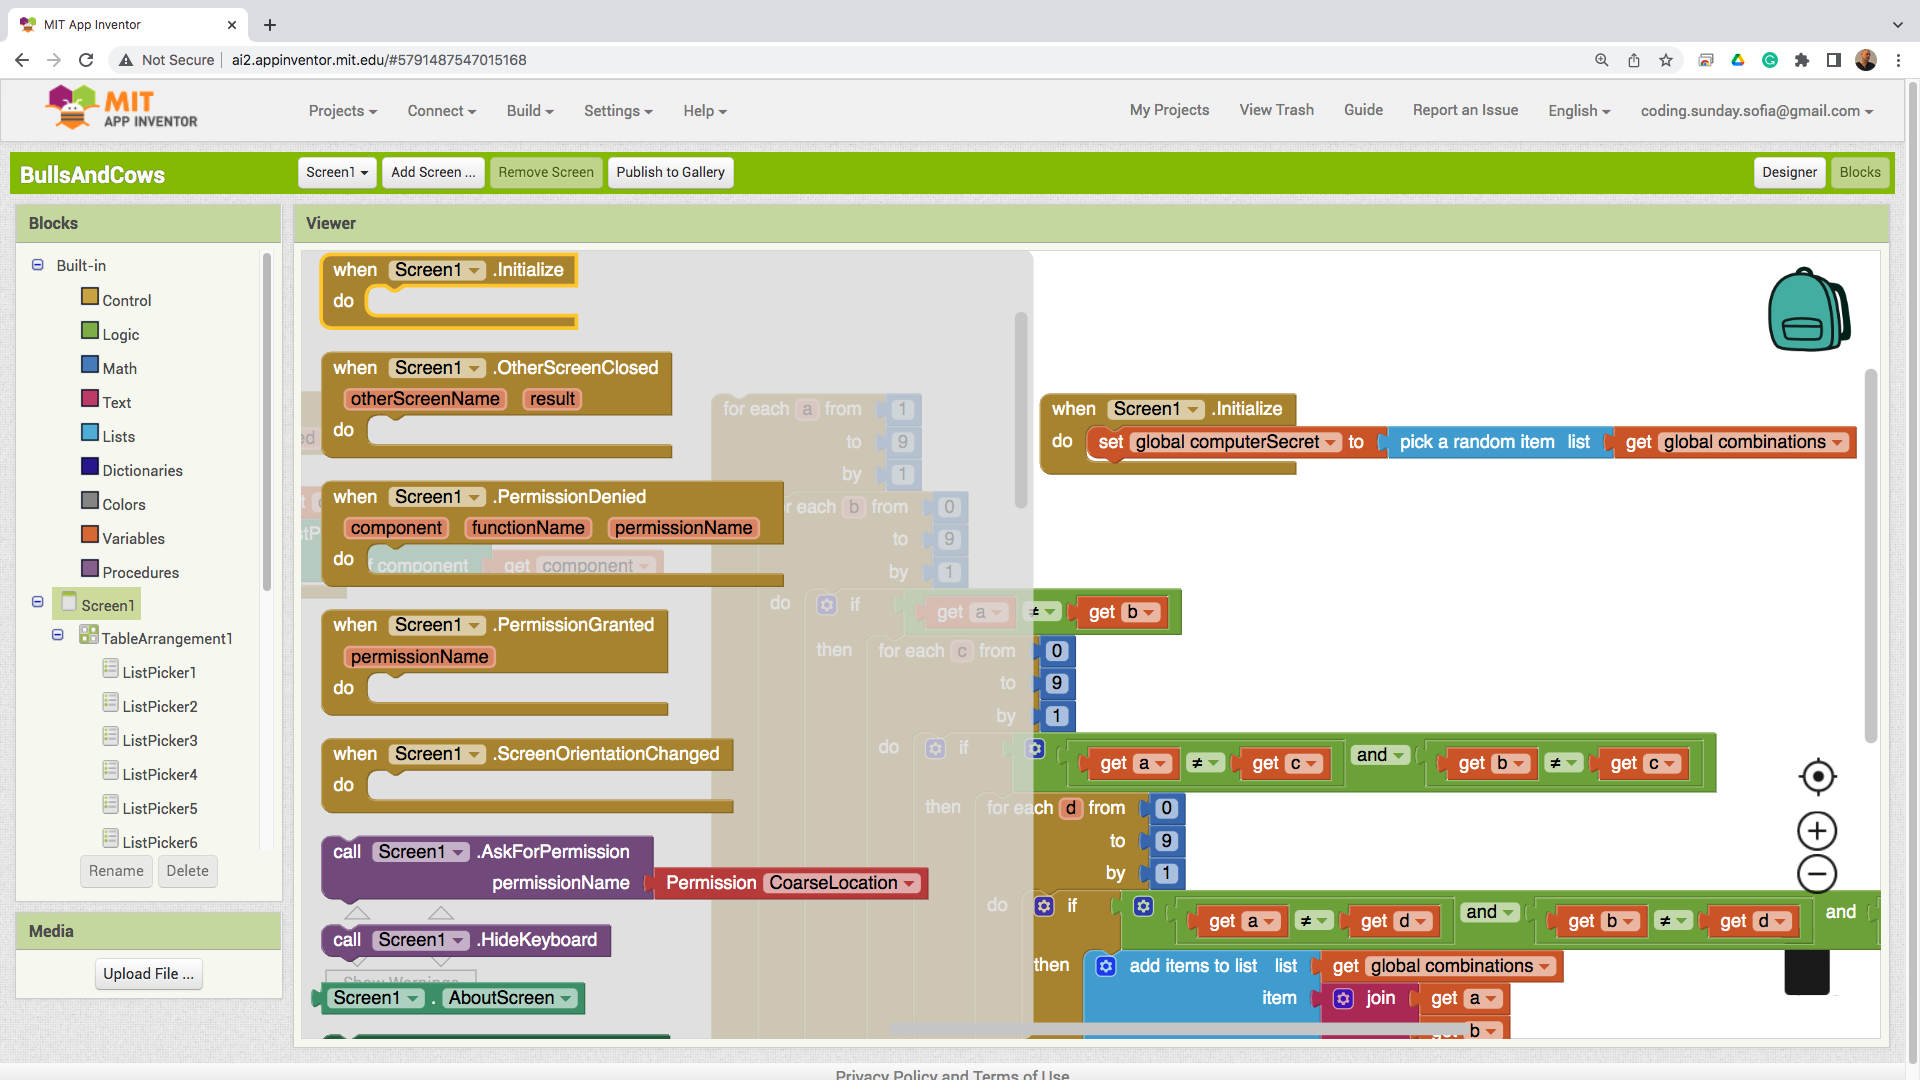
\includegraphics[width=1.0\linewidth,height=0.5\linewidth]{fig080014.png}
  \caption{Начална инициализация на екрана}
\label{fig080014}
\end{figure}

Задачата на първия бутон е да вземе предположение от компютърния опонент (извикване на допълнителна процедура) и да нулира всички останали цифри по визуалните компоненти (Фиг. \ref{fig080015}).

\begin{figure}[H]
  \centering
  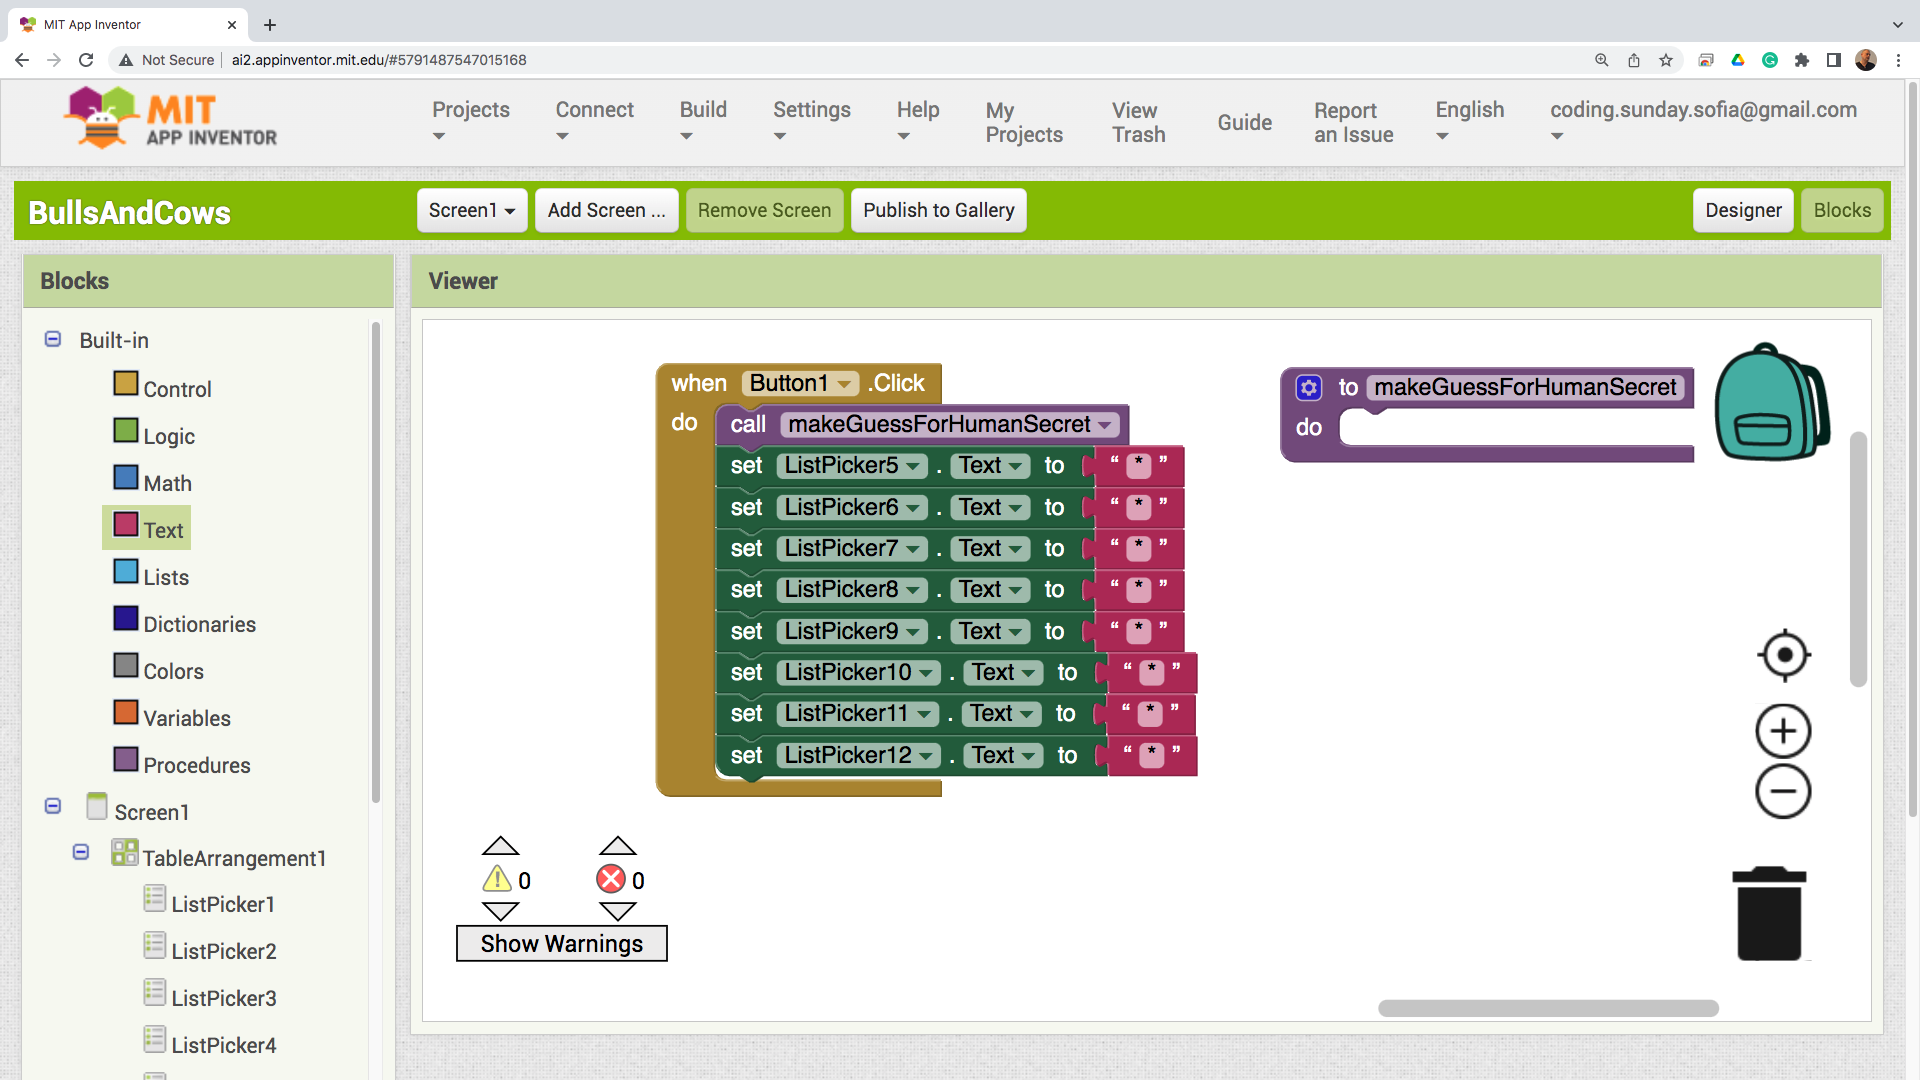
\includegraphics[width=1.0\linewidth,height=0.5\linewidth]{fig080015.png}
  \caption{Действия на първия бутон}
\label{fig080015}
\end{figure}

Компютърният опонент прави предположение за тайното число на играча, като избира един елемент от списъка с останали комбинации. Ако списъкът е празен (Фиг. \ref{fig080016}), то това означава, че човекът е подал неправилна информация на някой от предишните ходове и познаването на числото му е невъзможно. В компонент за нотификации се издава съобщение, че играта не може да продължи. 

\begin{figure}[H]
  \centering
  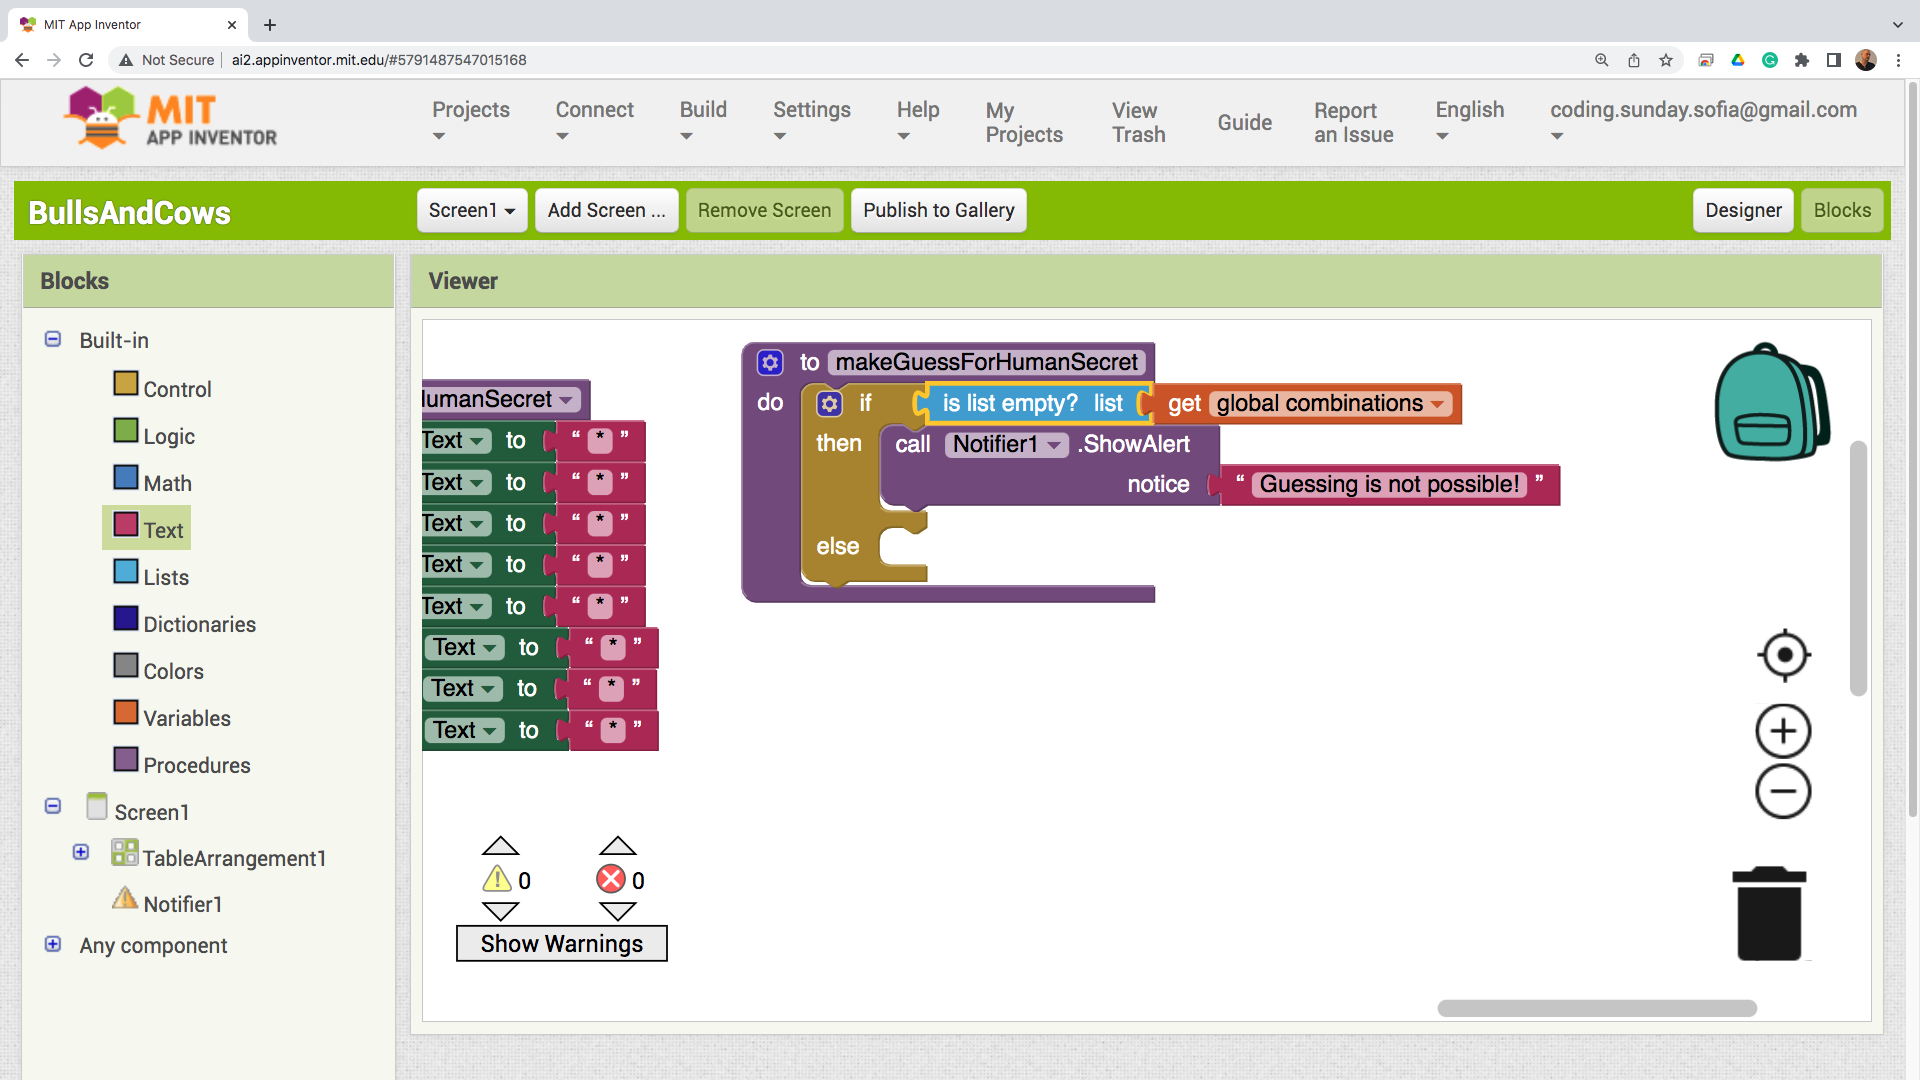
\includegraphics[width=1.0\linewidth,height=0.5\linewidth]{fig080016.png}
  \caption{Проверка за останали налични комбинации}
\label{fig080016}
\end{figure}

Ако в списъка с комбинации има елементи, то се избира един от елементите на случаен принцип (Фиг. \ref{fig080017}). Избраното число се визуализира в първите четири клетки от интерфейса, като за тази цел се вземат отделните цифри. 

\begin{figure}[H]
  \centering
  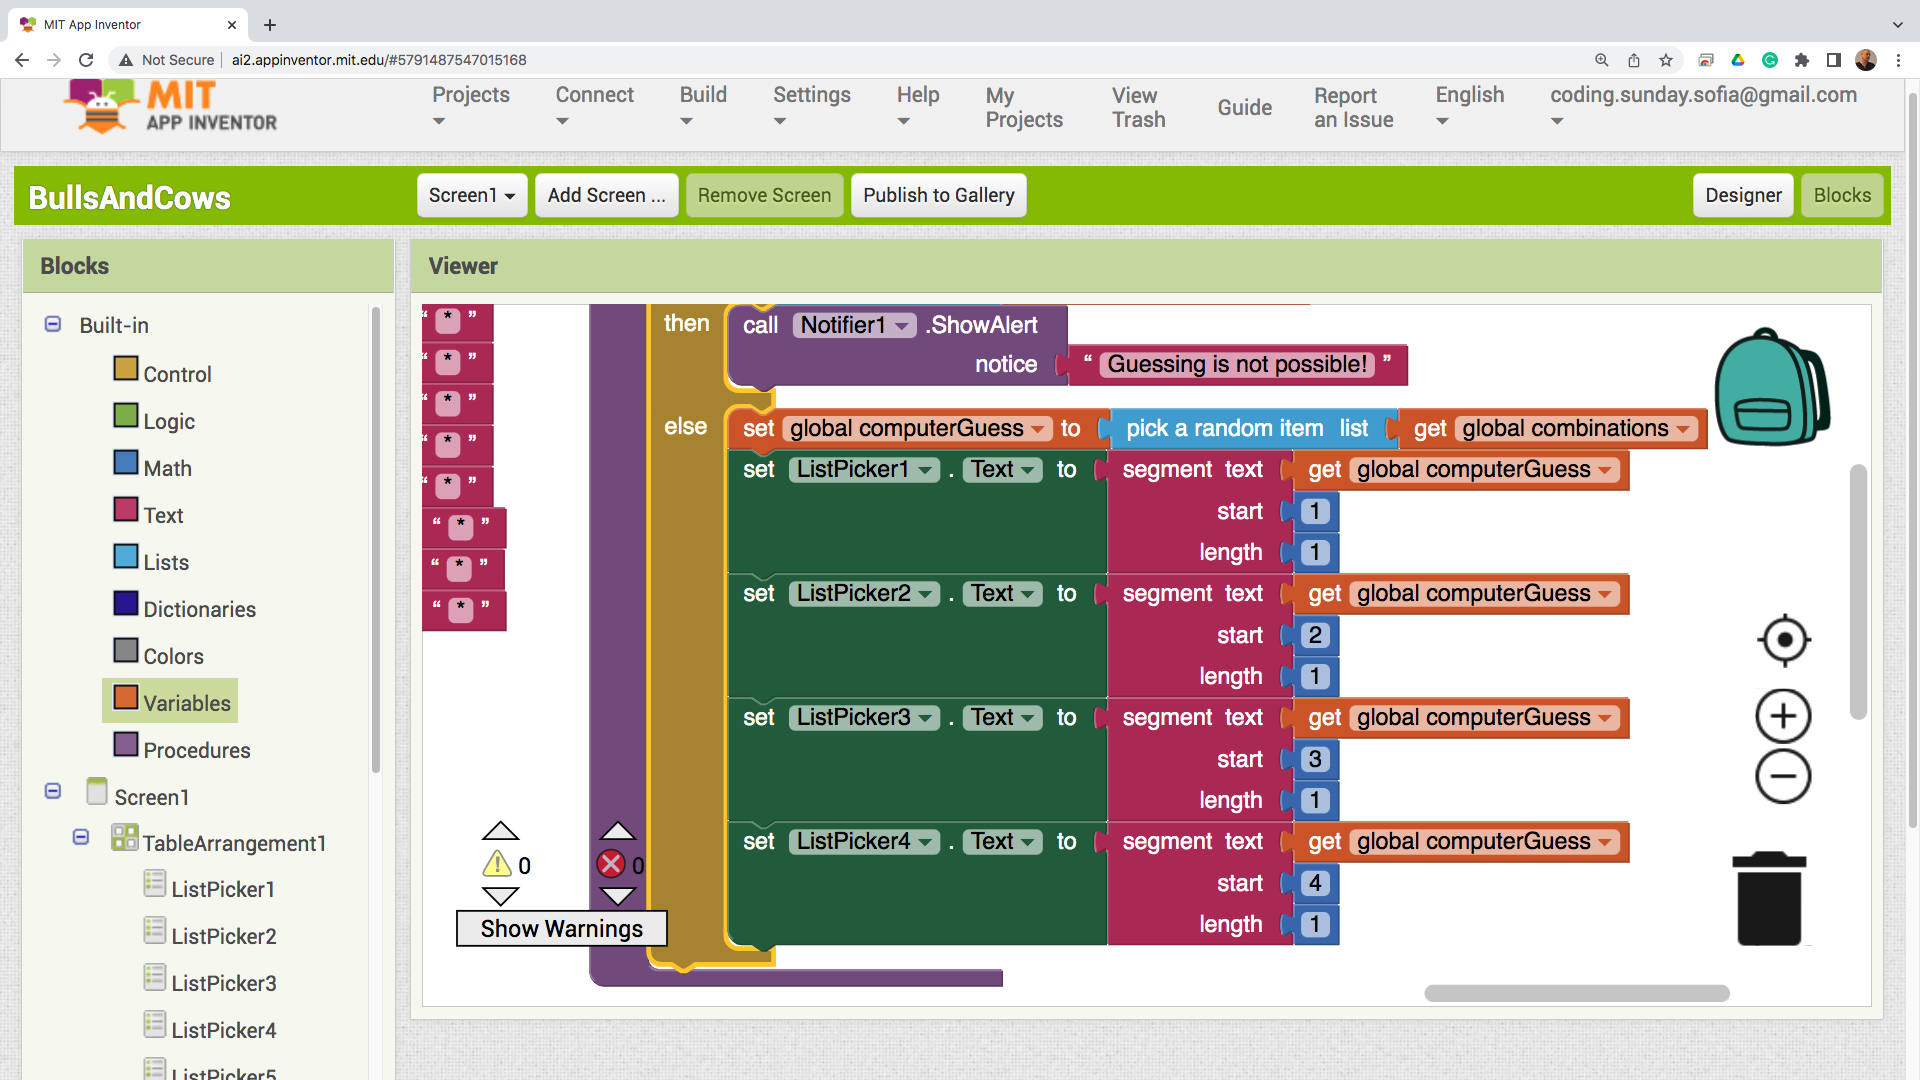
\includegraphics[width=1.0\linewidth,height=0.5\linewidth]{fig080017.png}
  \caption{Избор на число за предположение}
\label{fig080017}
\end{figure}

При натискането на втория бутон се изпълняват три действия, като за всяко от тях се извиква помощна процедура (Фиг. \ref{fig080018}). Първо се взема информацията от визуалните контроли, за предположението направено от човека. Второто действие е да се визуализират броя бикове и крави, уцелени от човека. Третото действие е да се изключат всички комбинации в списъка, които не отговарят на критериите от последното предположение, направено от компютърния опонент.

\begin{figure}[H]
  \centering
  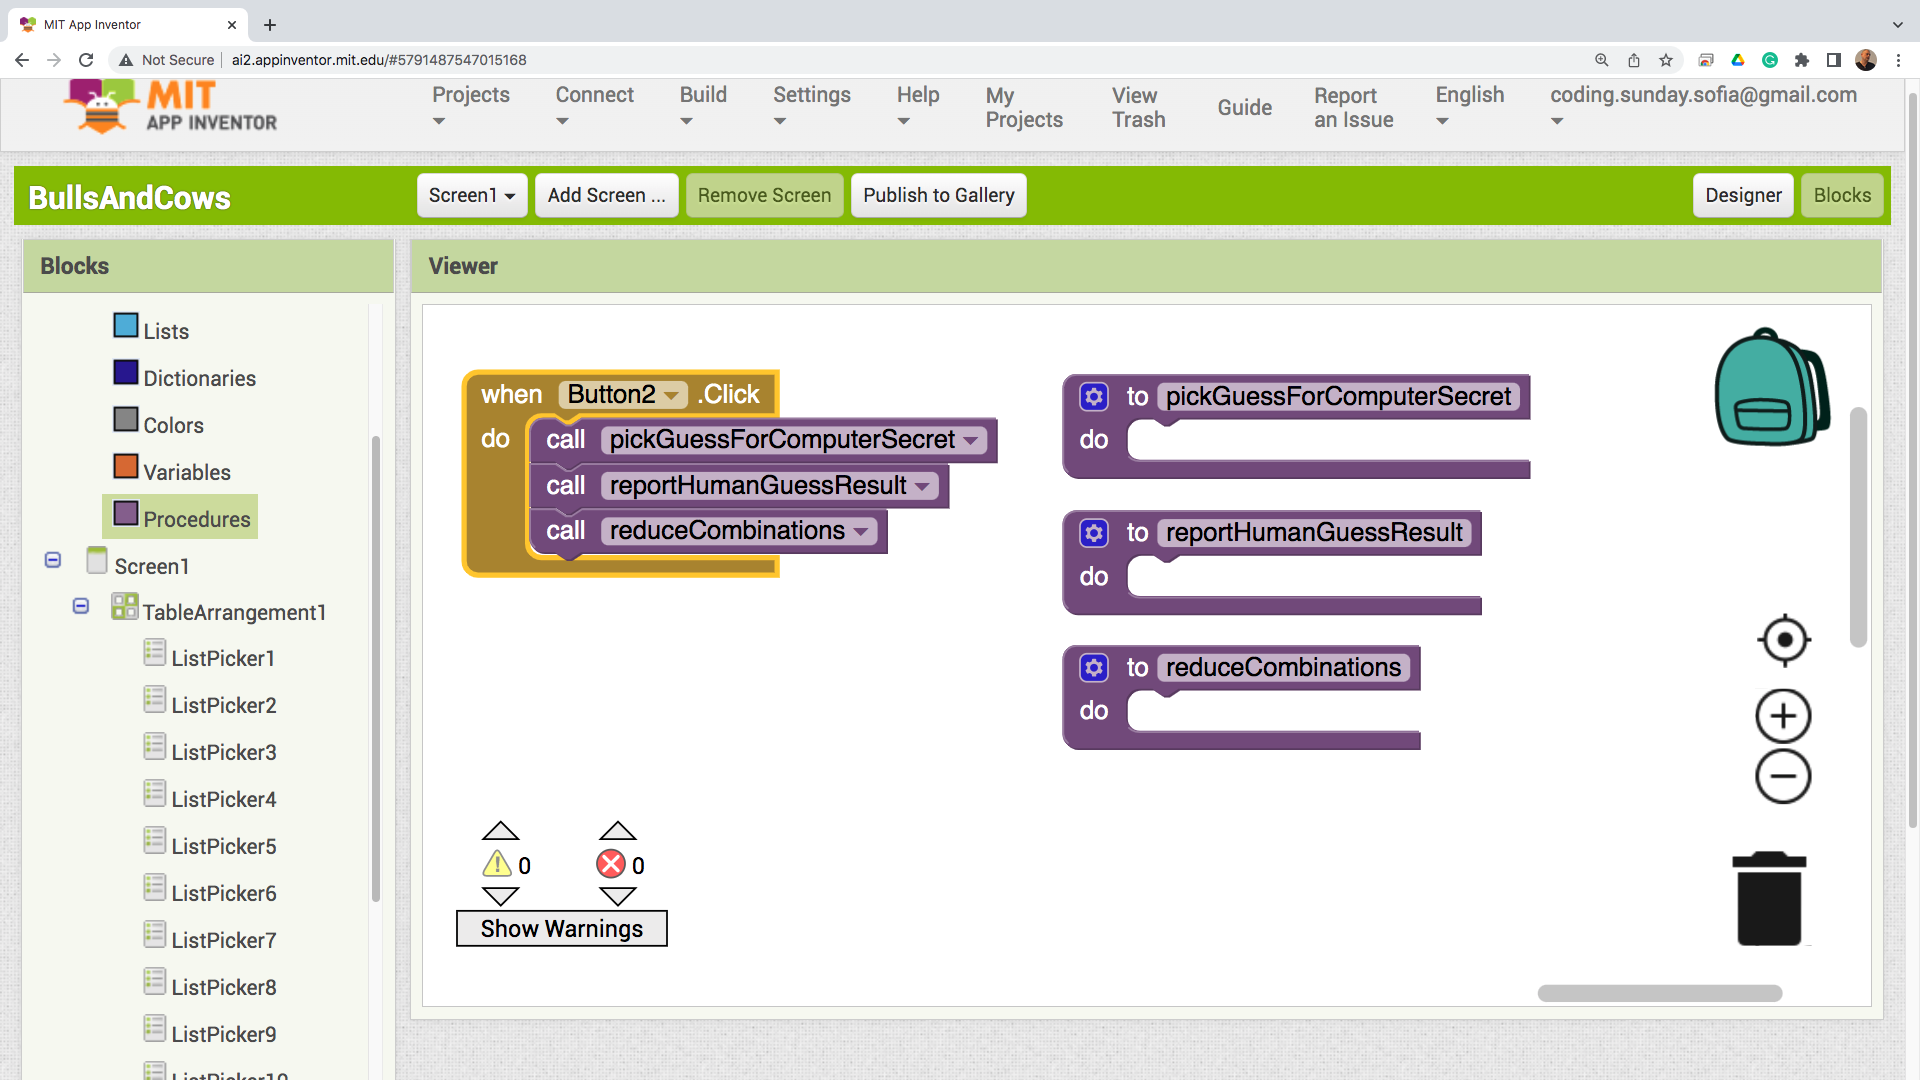
\includegraphics[width=1.0\linewidth,height=0.5\linewidth]{fig080018.png}
  \caption{Действия на първия бутон}
\label{fig080018}
\end{figure}

Предположението на човека се взема от визуалните контроли, като всяка от цифрите се слепва с останалите и се записва в помощната глобална променлива (Фиг. \ref{fig080019}).

\begin{figure}[H]
  \centering
  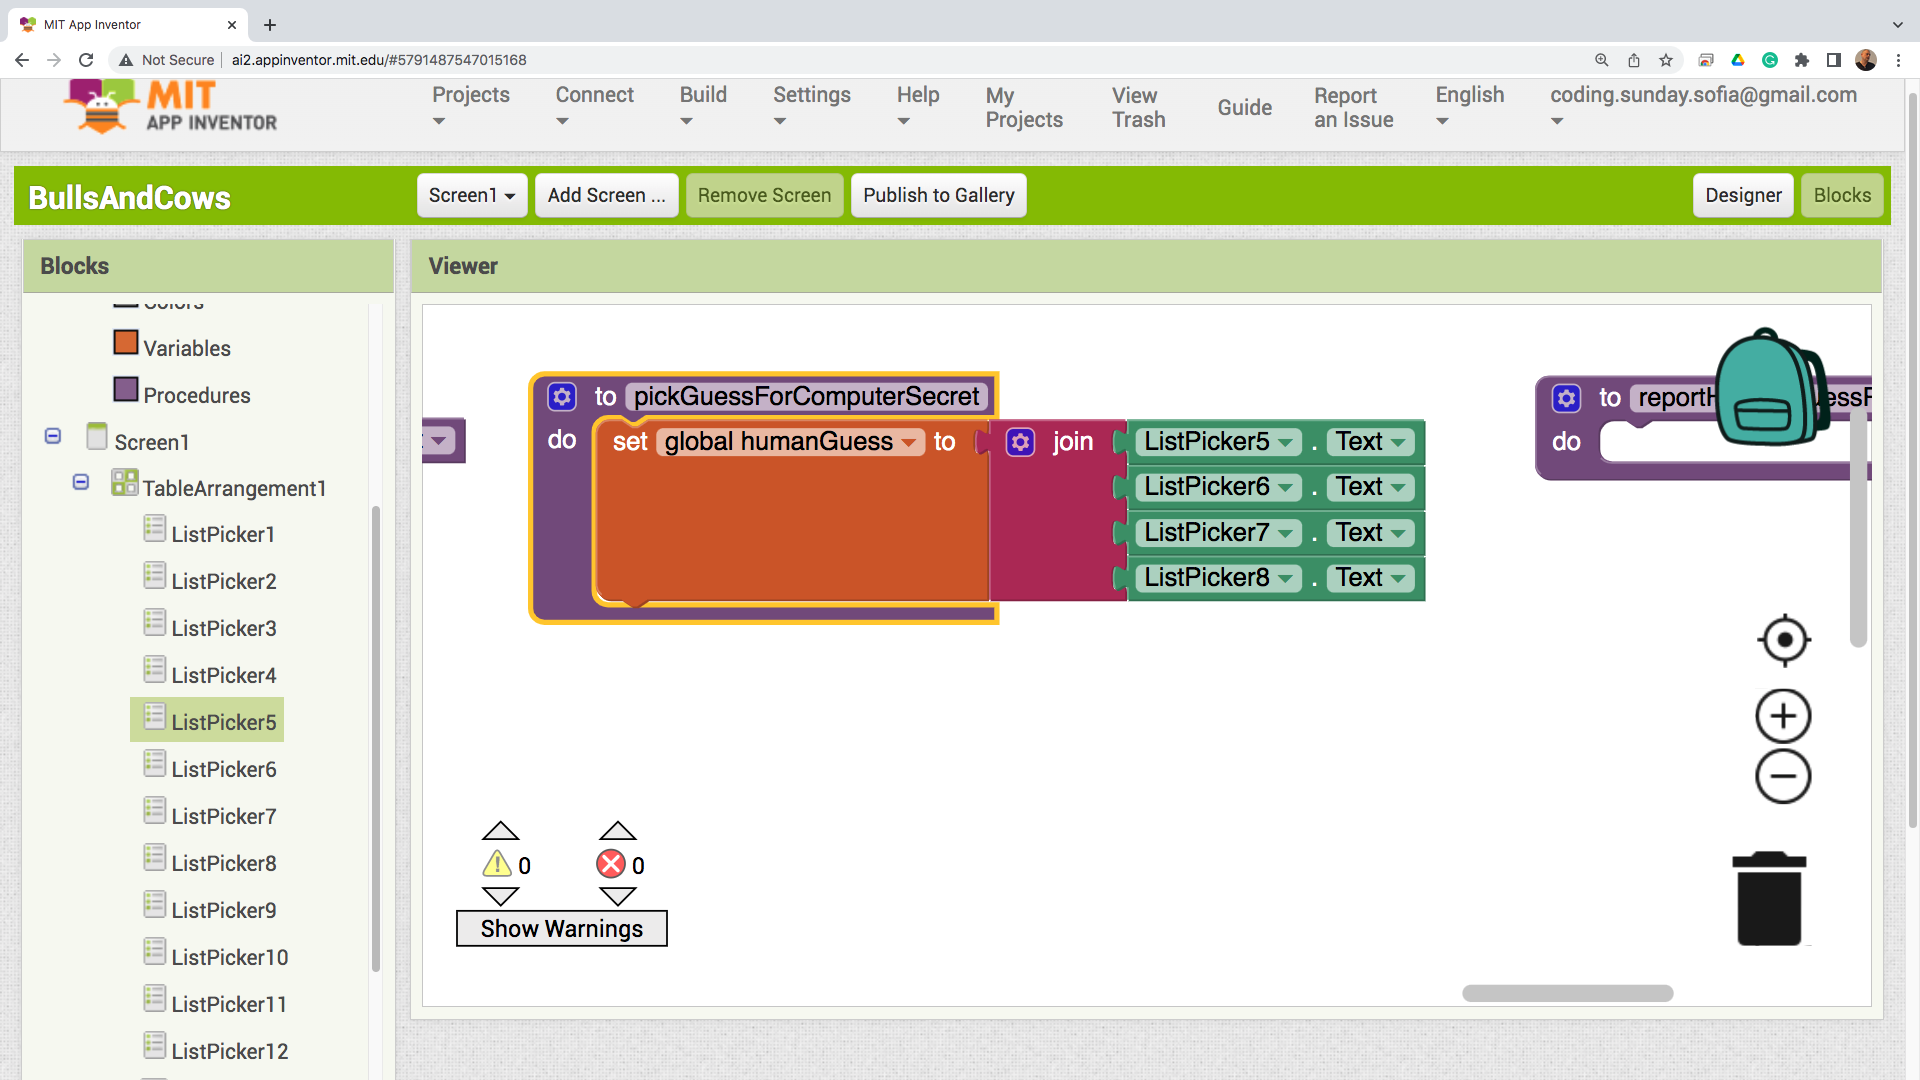
\includegraphics[width=1.0\linewidth,height=0.5\linewidth]{fig080019.png}
  \caption{Вземане на предположението от човека}
\label{fig080019}
\end{figure}

Броят познати бикове и крави от човека се определят с помощна процедура, която връща списък с два елемента. Първият елемент съдържа броя на биковете, а втория елемент броя на кравите. За да се изчислят тези бройки се използва тайното число на компютърния опонент и предположението, направено от играча (Фиг. \ref{fig080020}). Резултатът се показва в последните два компонента от графичния потребителски интерфейс.

\begin{figure}[H]
  \centering
  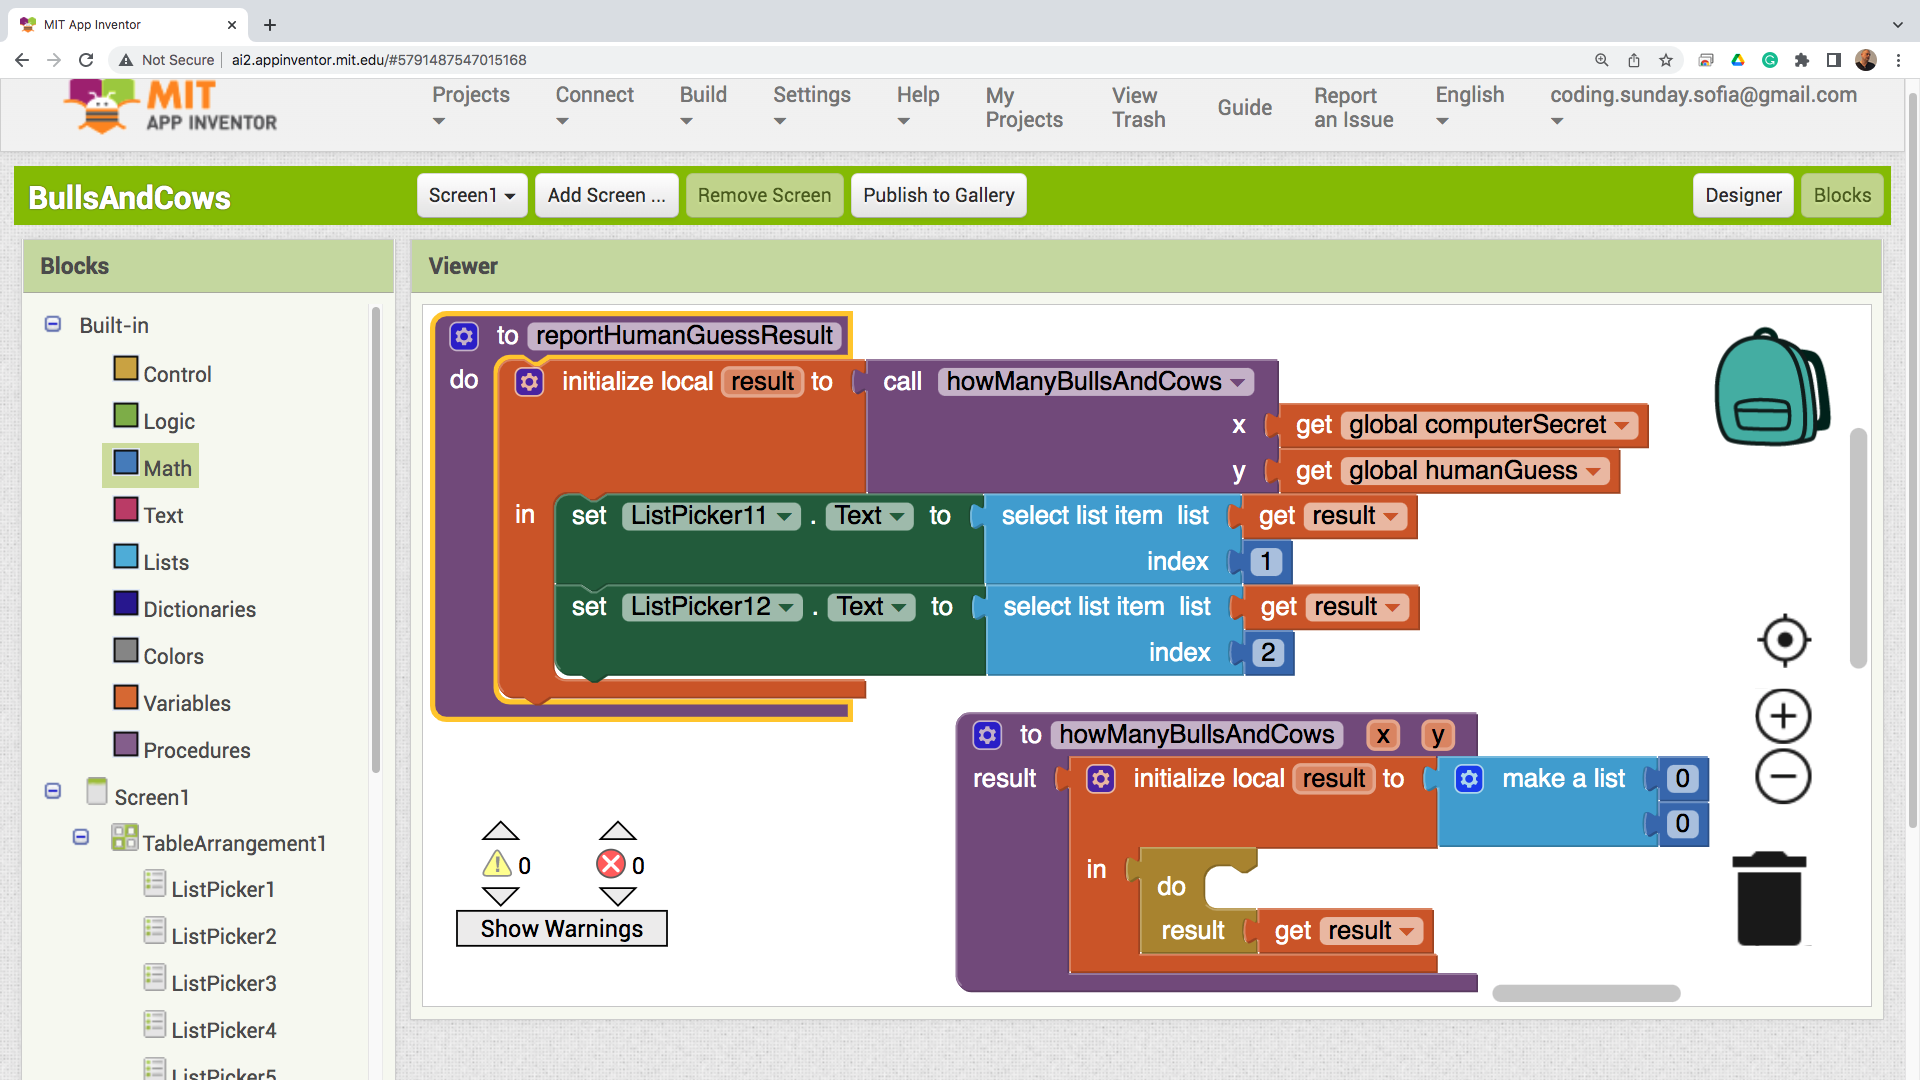
\includegraphics[width=1.0\linewidth,height=0.5\linewidth]{fig080020.png}
  \caption{Визуализация на броя бикове и крави познати от човека}
\label{fig080020}
\end{figure}

За да се редуцира броят на комбинациите, трябва да се вземе резултатът от проверката на направеното предположение, тоест броя бикове и крави, докладвани от човека. Това се постига с помощна процедура, която също връща списък, на който първият елемент съдържа броя бикове, а вторият елемент броя крави (Фиг. \ref{fig080021}).

\begin{figure}[H]
  \centering
  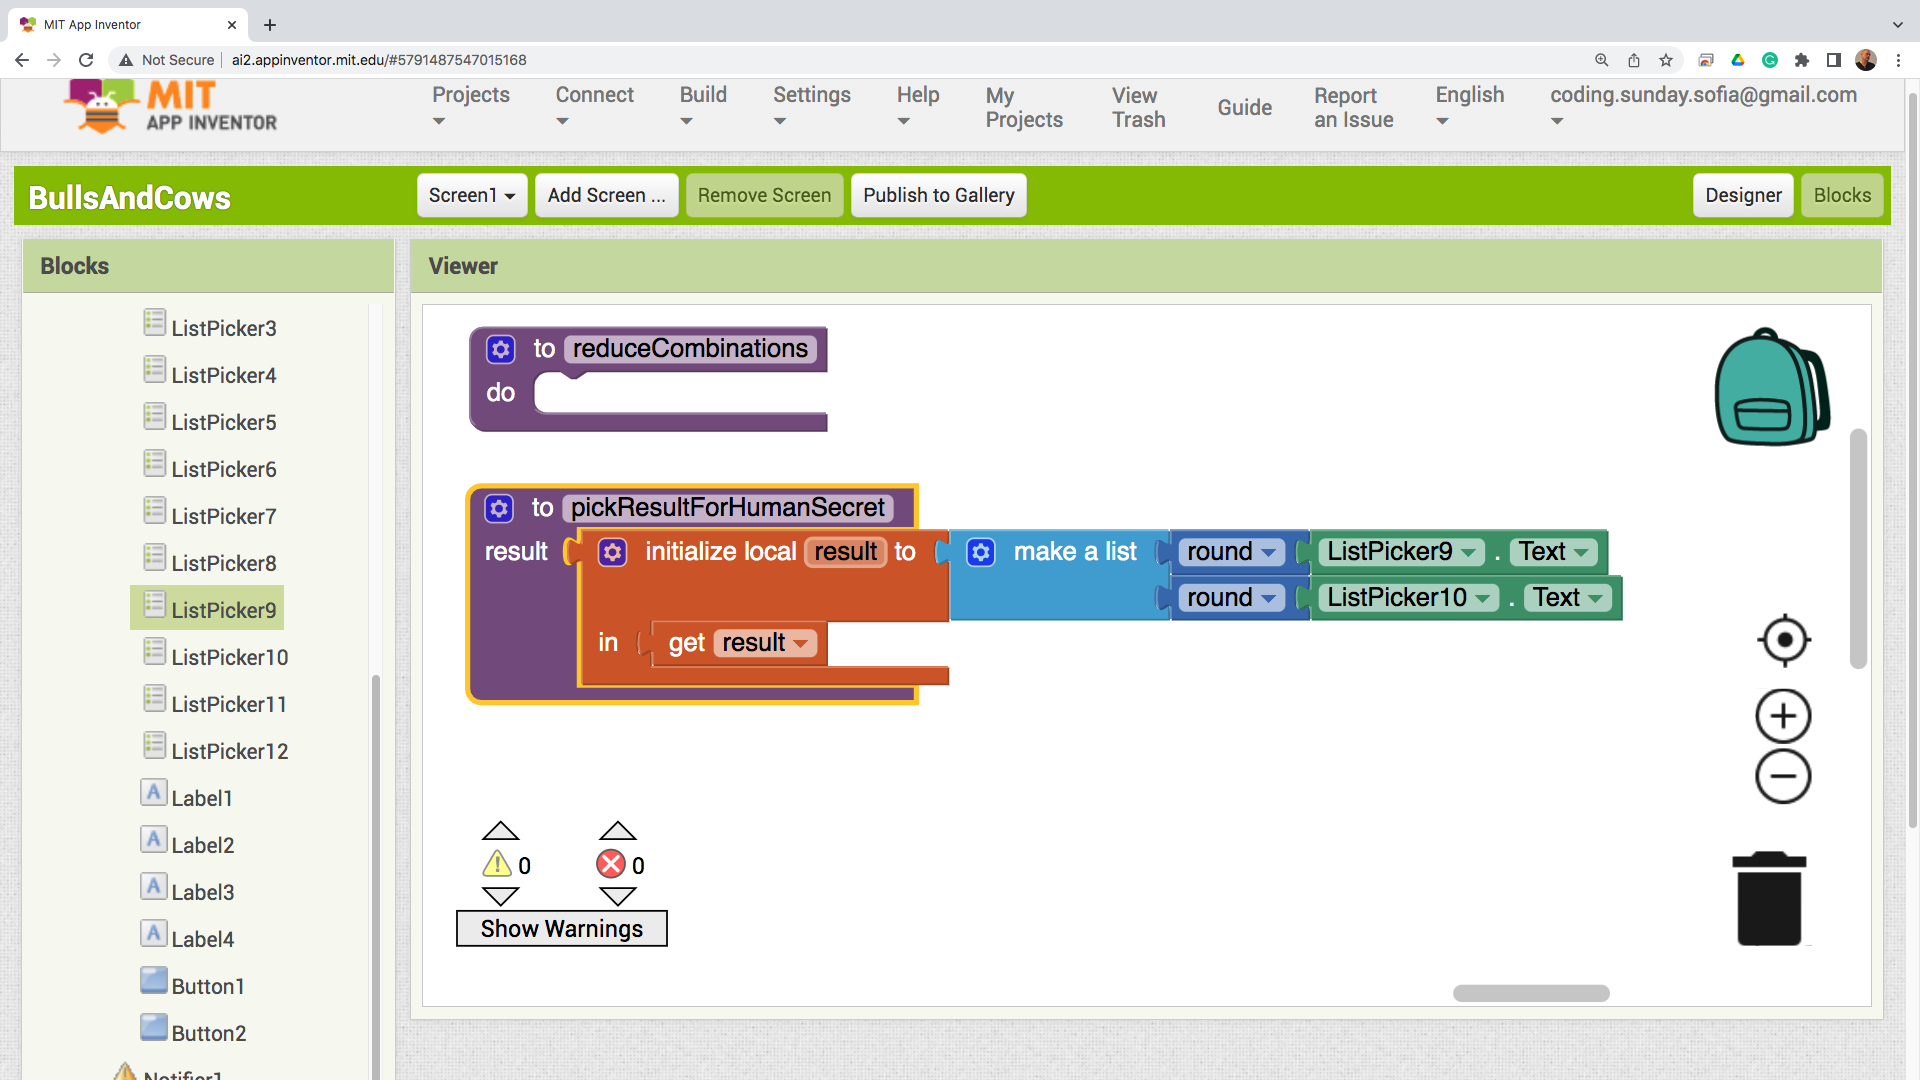
\includegraphics[width=1.0\linewidth,height=0.5\linewidth]{fig080021.png}
  \caption{Вземане на броя бикове и крави обявени от човека}
\label{fig080021}
\end{figure}

Отсяването на ненужните комбинации става чрез вземане на отговора, даден от човекът опонент. След това се създава нов празен списък, в който списък ще влязат само числата, които отговарят на посочените в отговора критерии. Отсяването се постига с прехождане на списъка с комбинации (Фиг. \ref{fig080022}). Всяка комбинация се подава на помощната функция, която да определи колко бика и крави формира комбинацията, спрямо предположението, направено от компютърния опонент. Ако текущо проверяваната комбинация има същите характеристики (брой бикове и брой крави), както са характеристиките, подадени в отговор от човека опонент, то текущата комбинация влиза в новия списък. След цялостното прехождане на списъка от комбинации, старият списък се подменя с новия списък.

\begin{figure}[H]
  \centering
  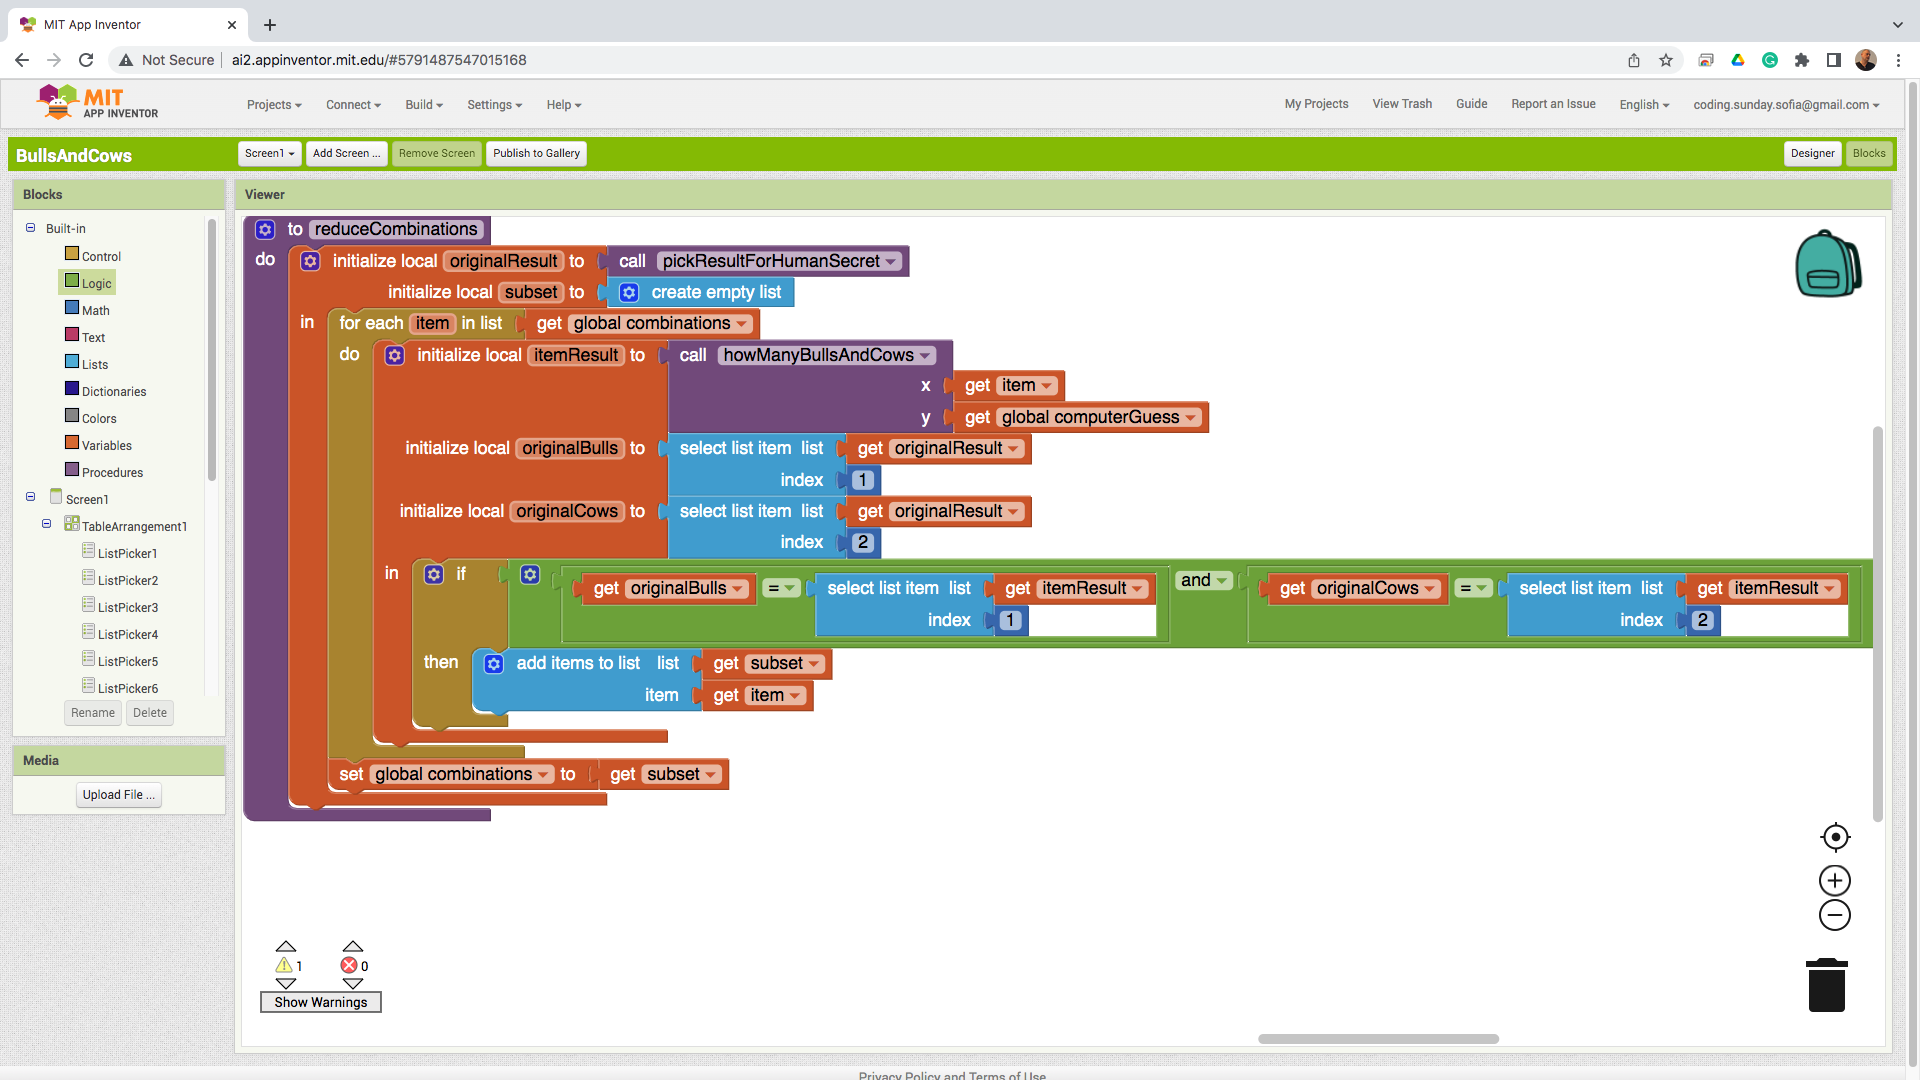
\includegraphics[width=1.0\linewidth,height=0.5\linewidth]{fig080022.png}
  \caption{Отсяване на ненужните комбинации}
\label{fig080022}
\end{figure}

Изчисляването на броя бикове и броя крави, за две числа става, чрез завъртането на два цикъла. Единият цикъл обхожда първото число, цифра по цифра, а вторият цикъл второто число, пак цифра по цифра (Фиг. \ref{fig080023}).

\begin{figure}[H]
  \centering
  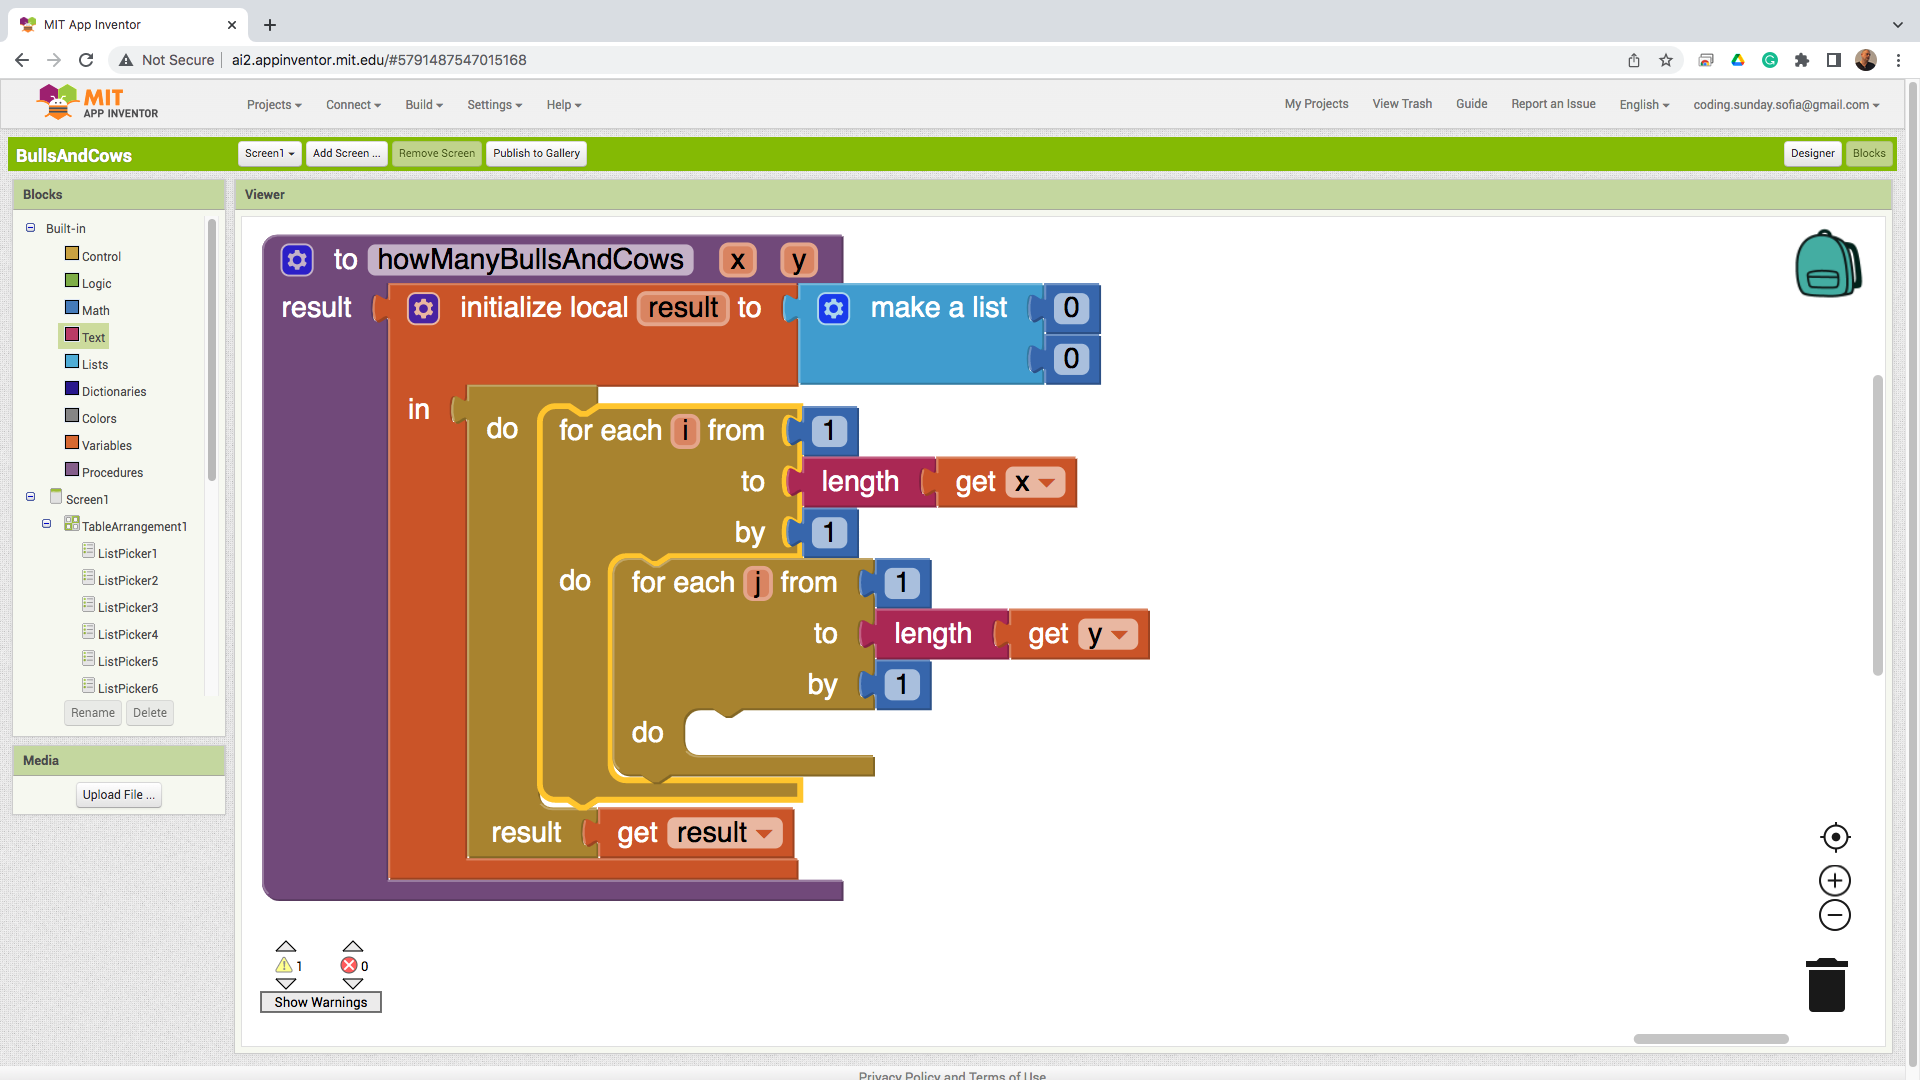
\includegraphics[width=1.0\linewidth,height=0.5\linewidth]{fig080023.png}
  \caption{Обхождане на цифрите на две числа}
\label{fig080023}
\end{figure}

Текущо разглежданите цифри на двете числа се зареждат в две помощни променливи (Фиг. \ref{fig080024}). С тези две променливи и с броячите на циклите се правят нужните сравнения за наличие на бик или крава. 

\begin{figure}[H]
  \centering
  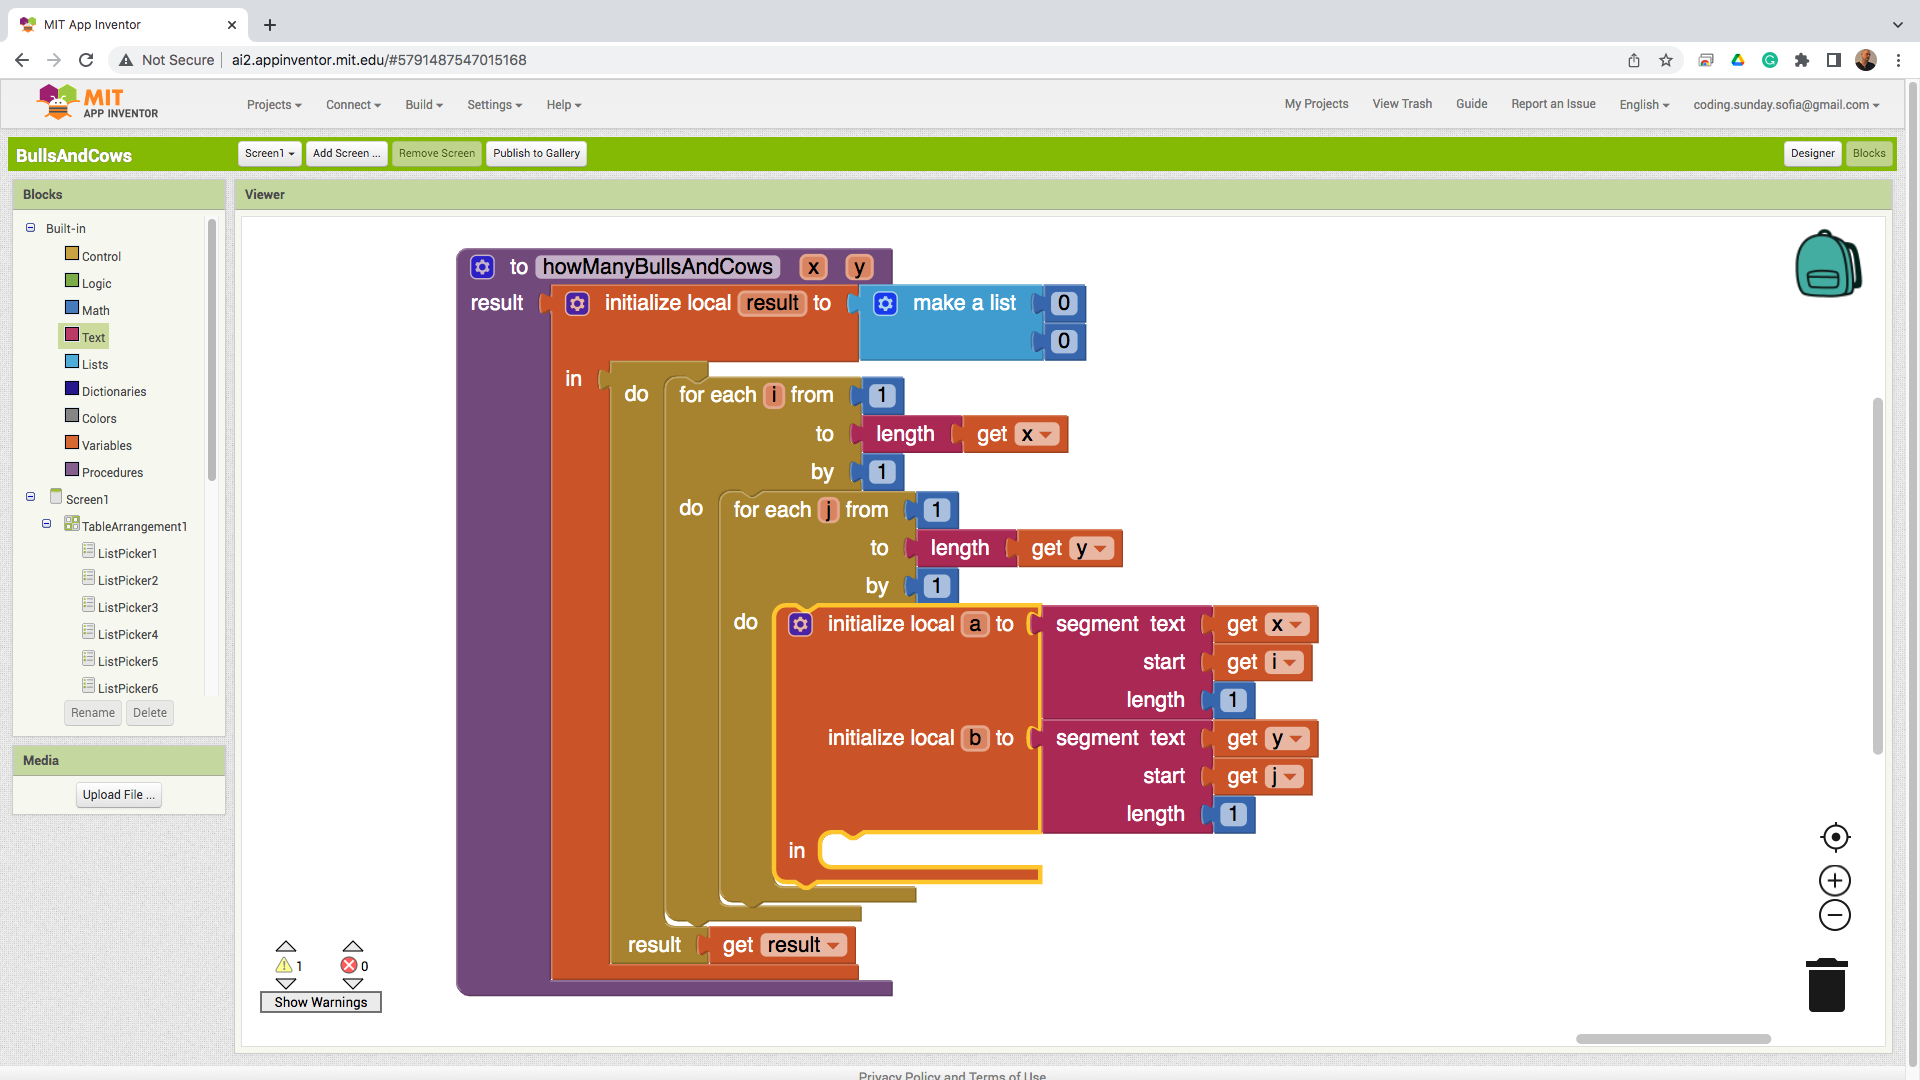
\includegraphics[width=1.0\linewidth,height=0.5\linewidth]{fig080024.png}
  \caption{Помощни променливи за цифрите}
\label{fig080024}
\end{figure}

Ако двете цифри съвпадат, то това означава или бик или крава (Фиг. \ref{fig080025}). Дали съвпадението е бик или крава се определя от стойностите на броячите за двата цикъла.

\begin{figure}[H]
  \centering
  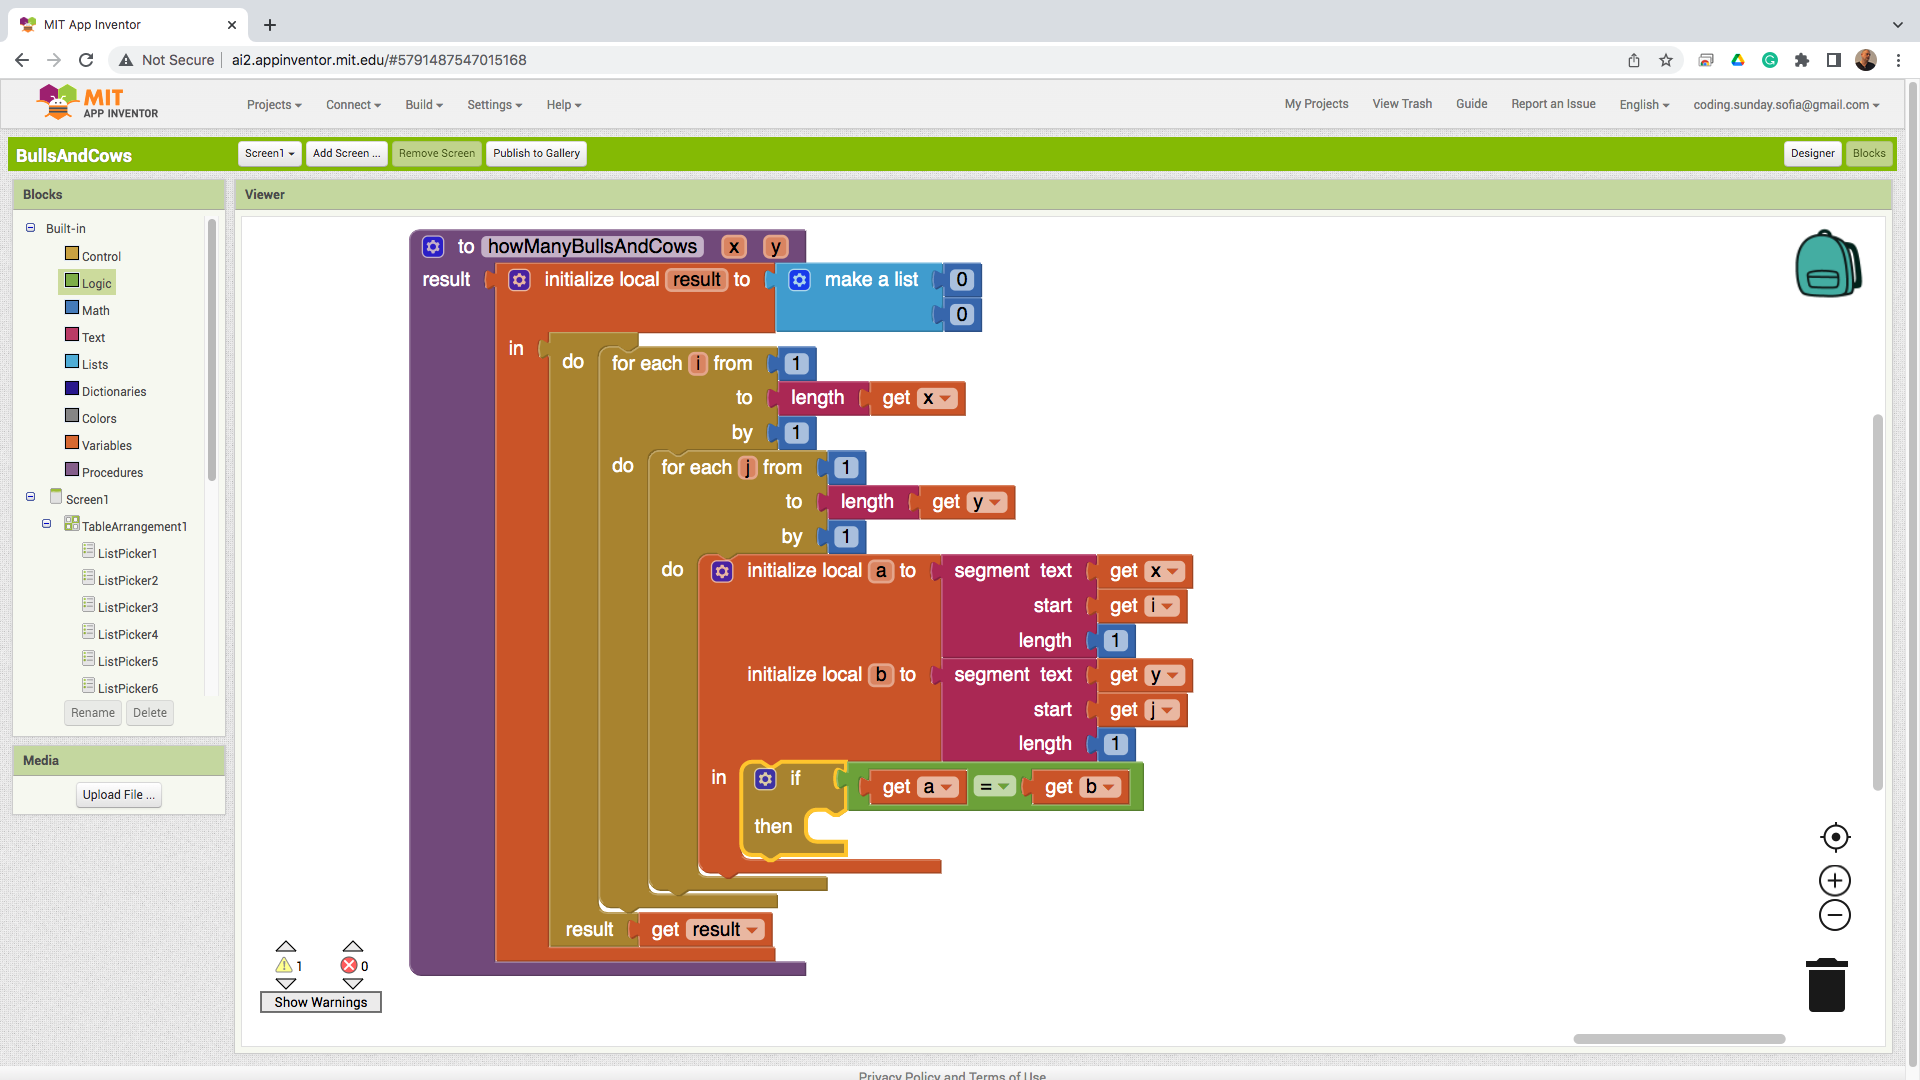
\includegraphics[width=1.0\linewidth,height=0.5\linewidth]{fig080025.png}
  \caption{Съвпадение на цифрите}
\label{fig080025}
\end{figure}

Ако двата брояча са с една и съща стойност, то е налице бик, в противен случай е на лице крава (Фиг. \ref{fig080026}).

\begin{figure}[H]
  \centering
  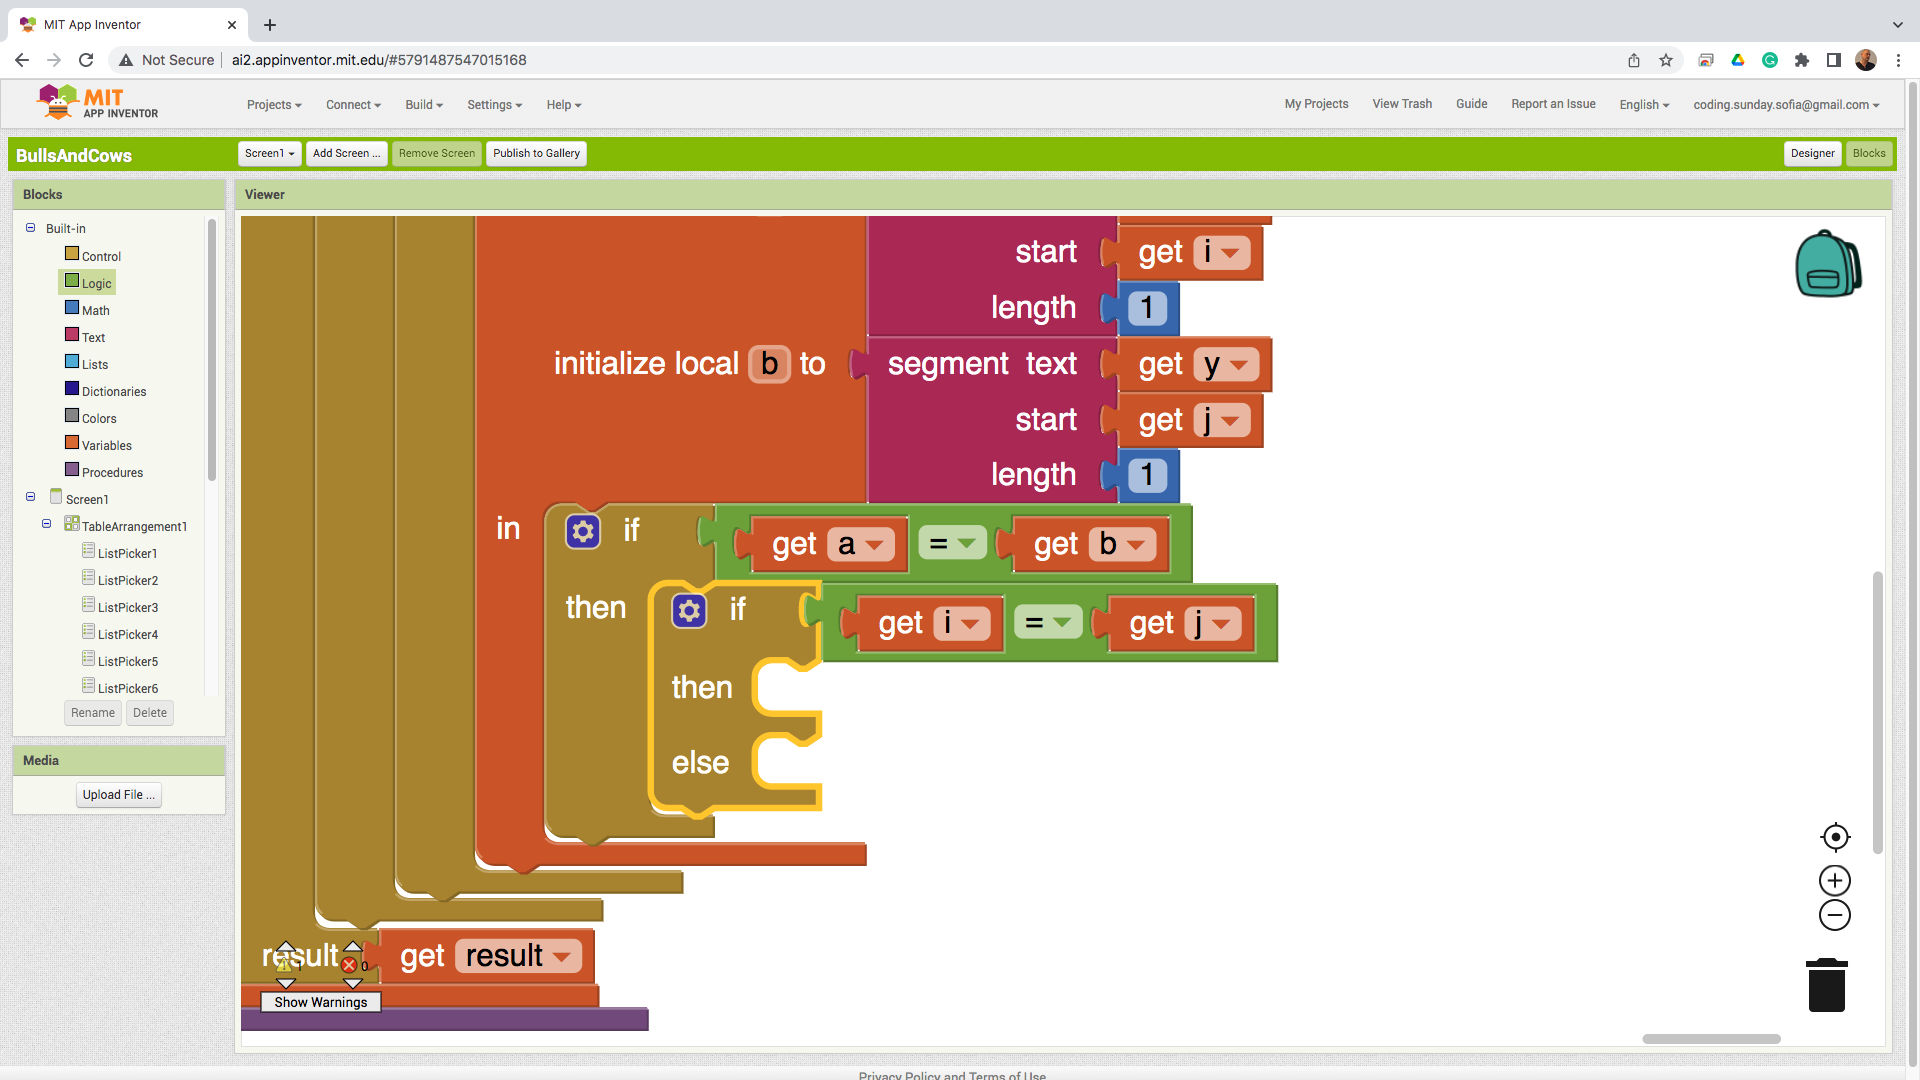
\includegraphics[width=1.0\linewidth,height=0.5\linewidth]{fig080026.png}
  \caption{Съвпадение на броячите}
\label{fig080026}
\end{figure}

При срещането на бик се увеличава с единица стойността на първия елемент в резултата, а при срещането на крава се увеличава с единица вторият елемент на списъка с резултата (Фиг. \ref{fig080027}).

\begin{figure}[H]
  \centering
  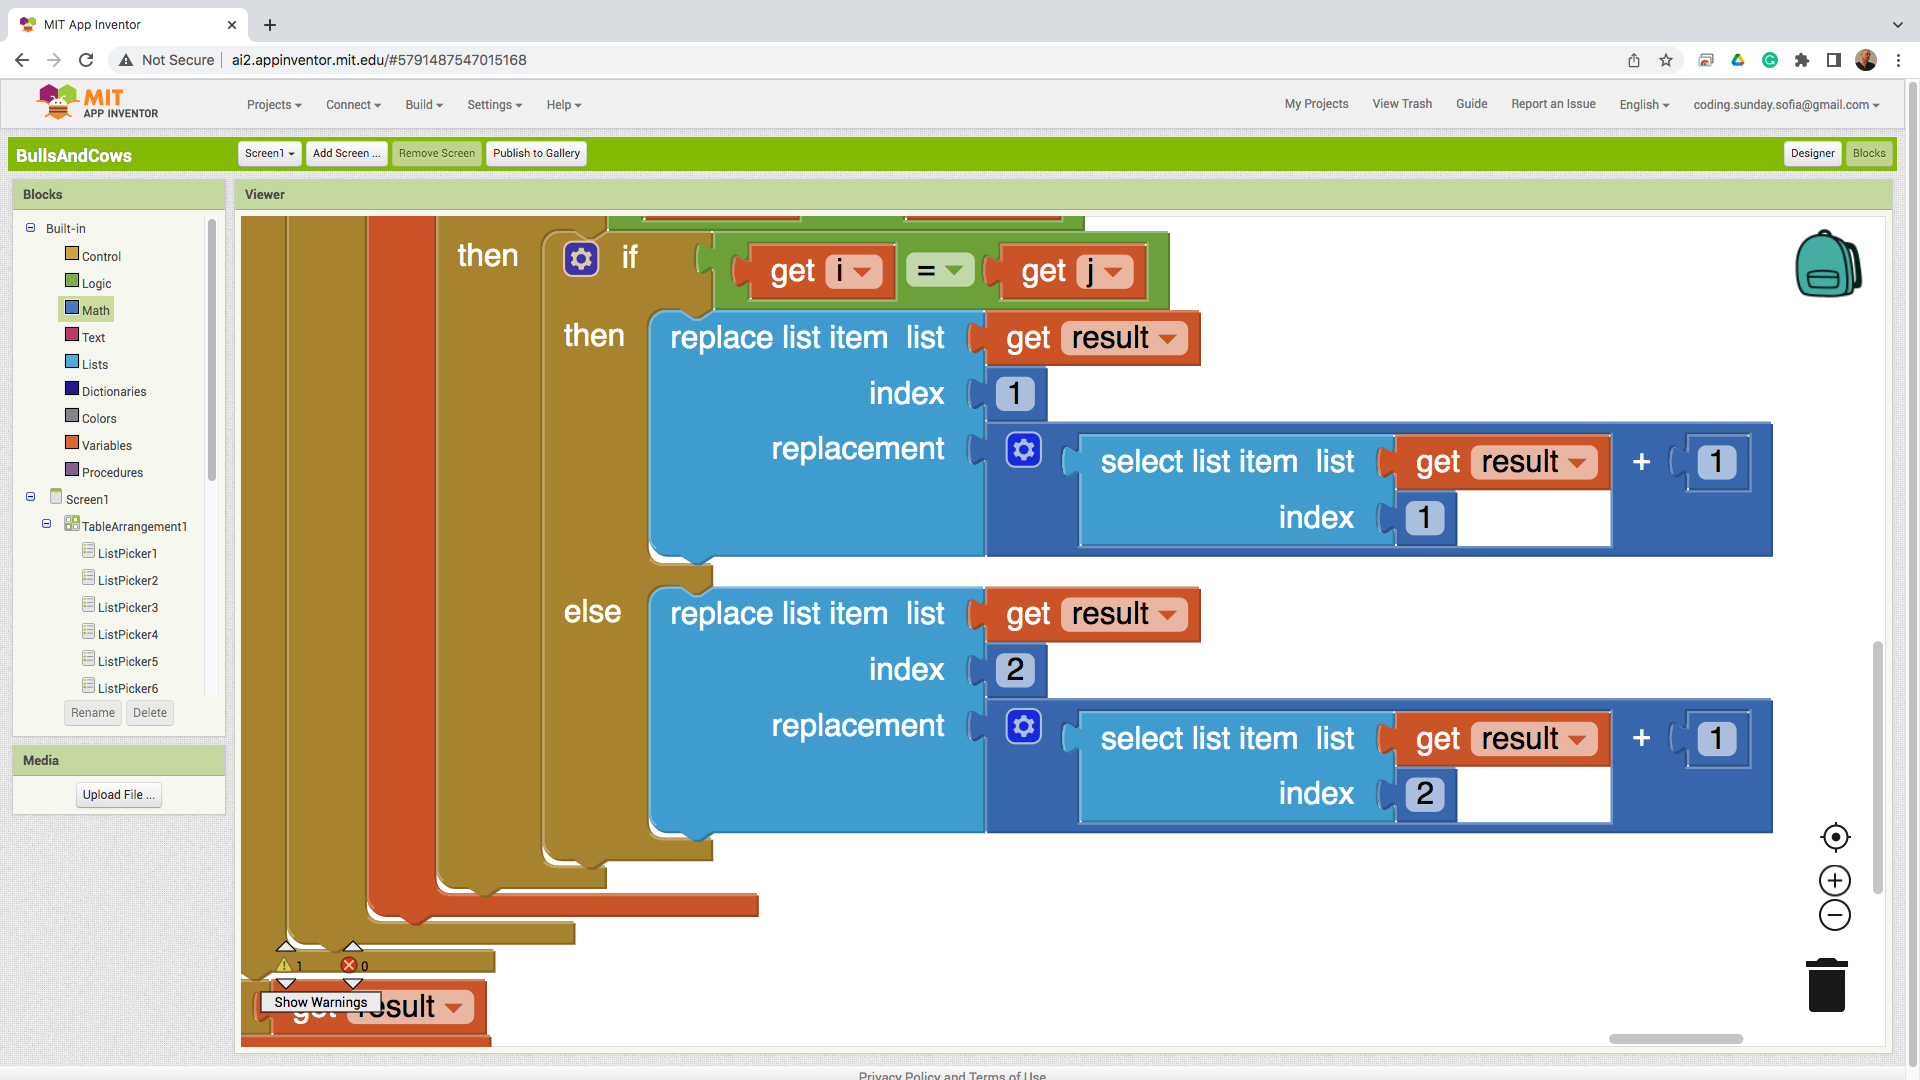
\includegraphics[width=1.0\linewidth,height=0.5\linewidth]{fig080027.png}
  \caption{Отброяване на биковете и кравите}
\label{fig080027}
\end{figure}

Играта се играе в последователност (Фиг. \ref{fig080028}), като първо се натисне първият бутон. Натискането на първия бутон дава възможност на компютърния опонент да направи предположение за тайното число на човека опонент. След това, човекът маркира колко бика и колко крави е успял да познае компютърният опонент. Третата стъпка е човекът опонент да направи своето предположение за тайното число на компютърния опонент. Следва натискане на втория бутон, при който компютърният опонент съобщава колко бика и колко крави е познал човекът. 

\begin{figure}[H]
  \centering
  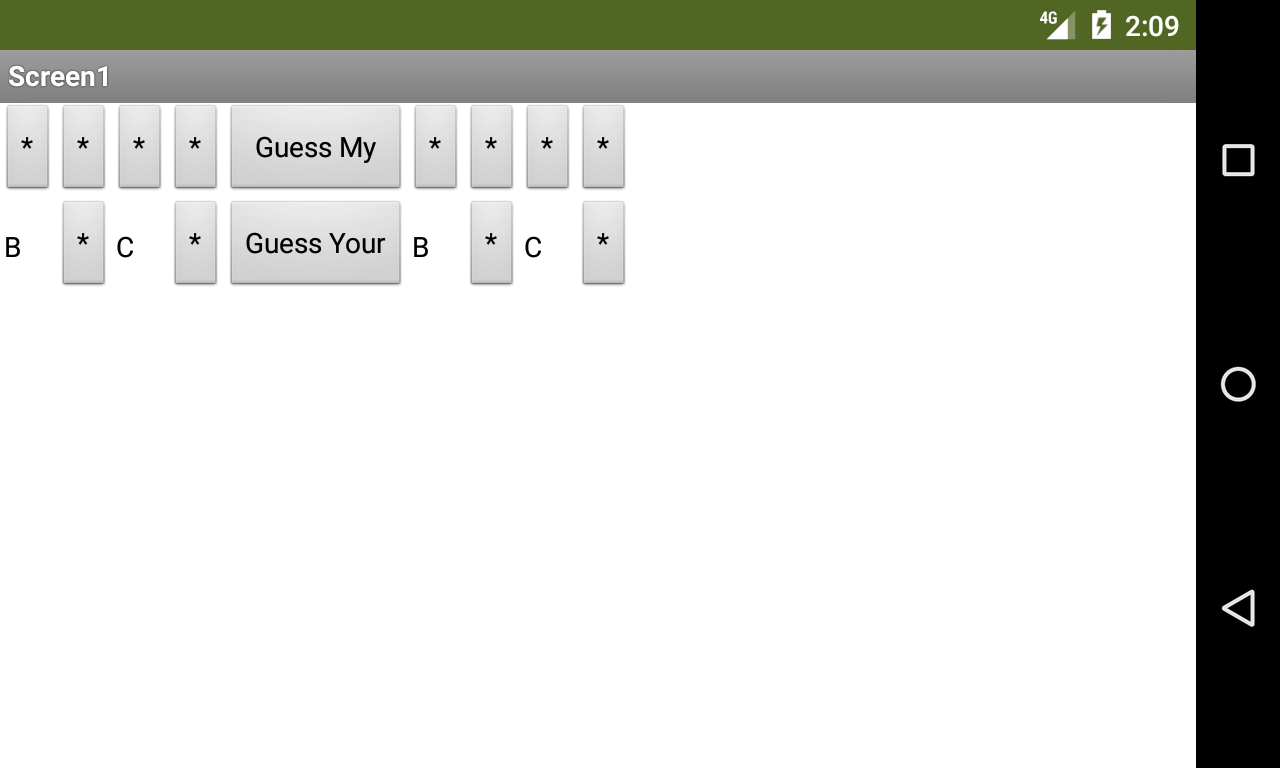
\includegraphics[width=1.0\linewidth,height=0.5\linewidth]{fig080028.png}
  \caption{Начален екран на играта}
\label{fig080028}
\end{figure}

Чрез следване на последователността от стъпки за работа с графичния интерфейс (Фиг. \ref{fig080029}), играта продължава докато един от играчите уцели четири бика.

\begin{figure}[H]
  \centering
  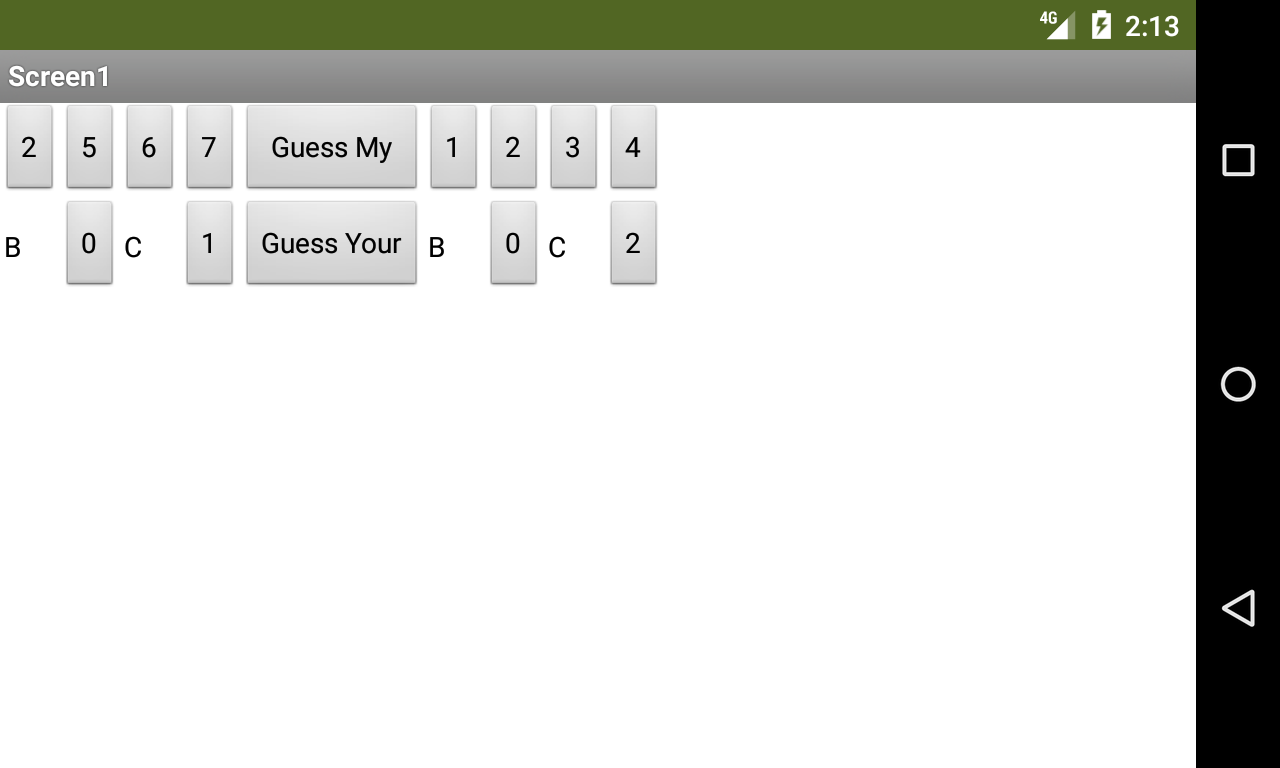
\includegraphics[width=1.0\linewidth,height=0.5\linewidth]{fig080029.png}
  \caption{Междинен ход в играта}
\label{fig080029}
\end{figure}

\section{Публикуване на проекта}

След достигане на пълнофункционален вариант на играта, проектът може да бъде публикуван в галерията, така че да бъде достъпен за широката аудитория (Фиг. \ref{fig080030}).

\begin{figure}[H]
  \centering
  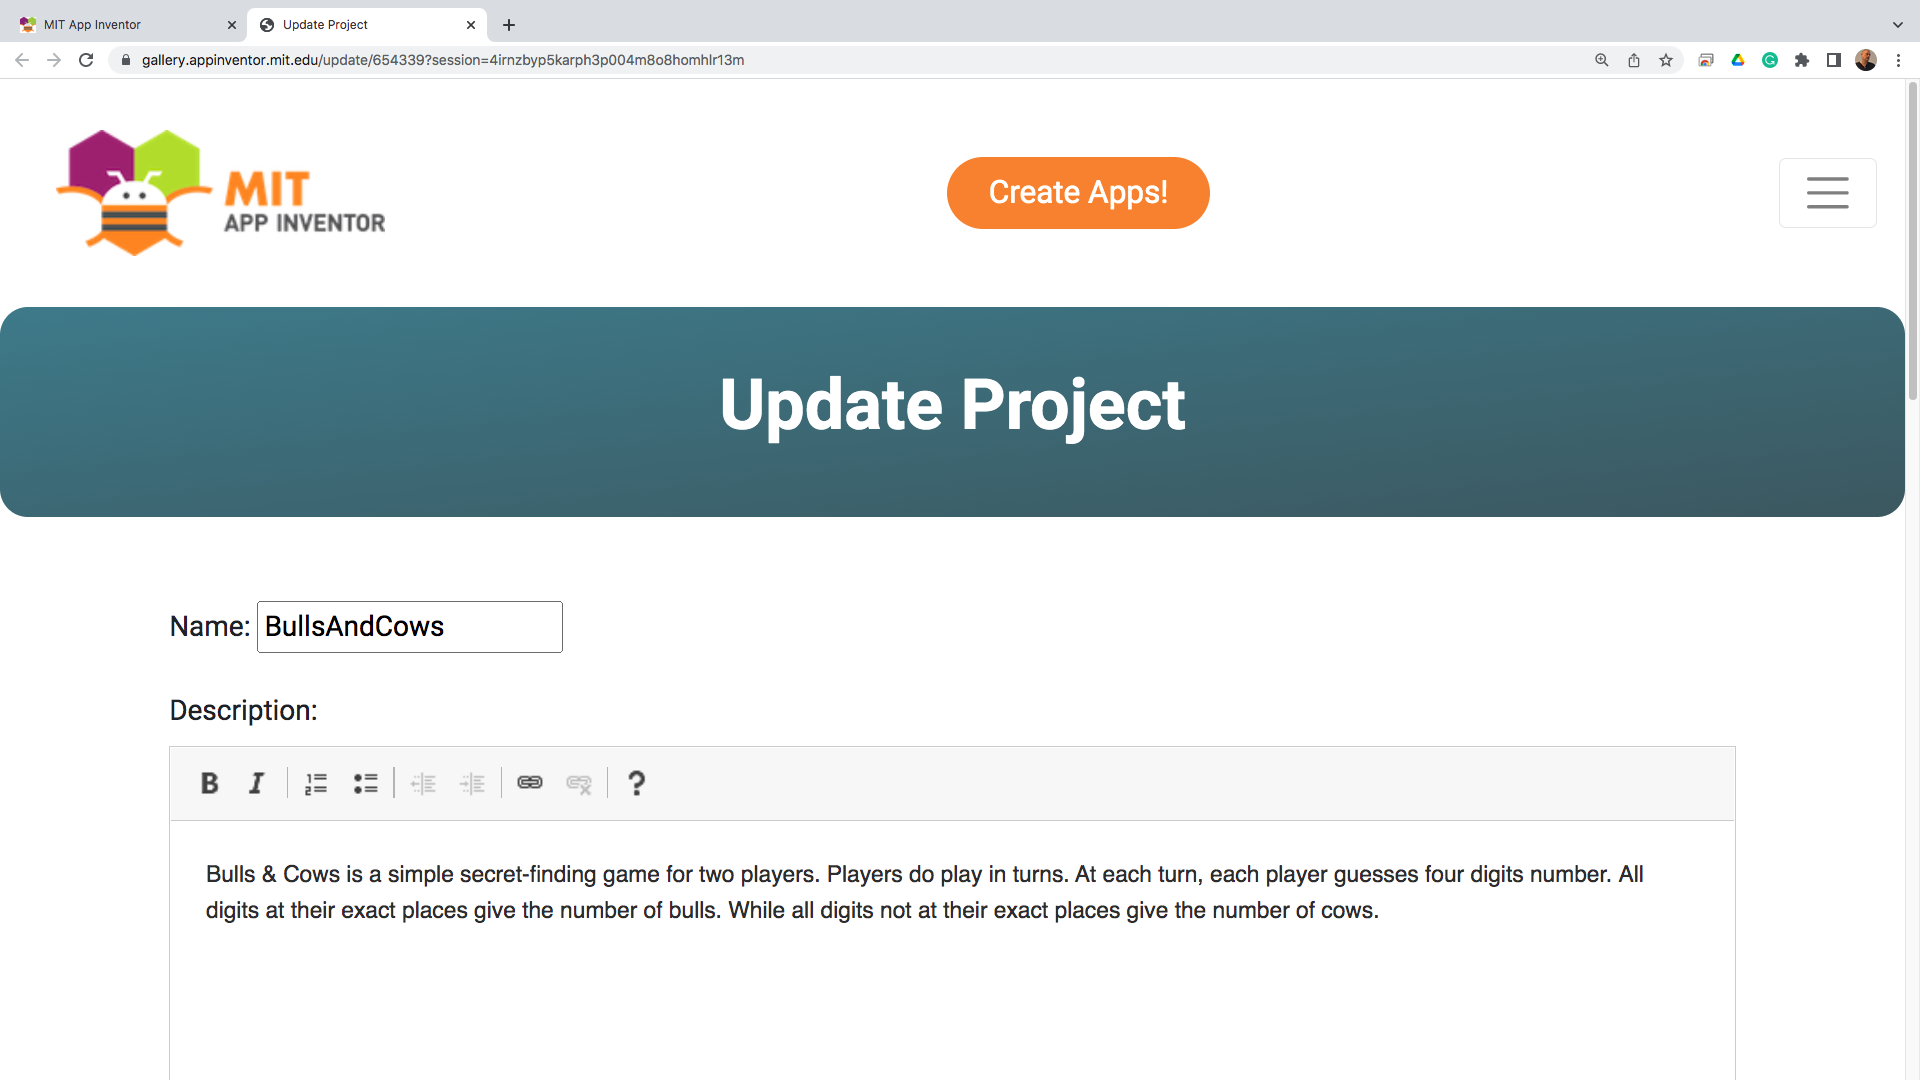
\includegraphics[width=1.0\linewidth,height=0.5\linewidth]{fig080030.png}
  \caption{Описание на проекта}
\label{fig080030}
\end{figure}

След публикуването, в страницата на приложението се появяват хипервръзки за стартиране на програмата или разглеждане на кода й в развойната среда (Фиг. \ref{fig080031}).

\begin{figure}[H]
  \centering
  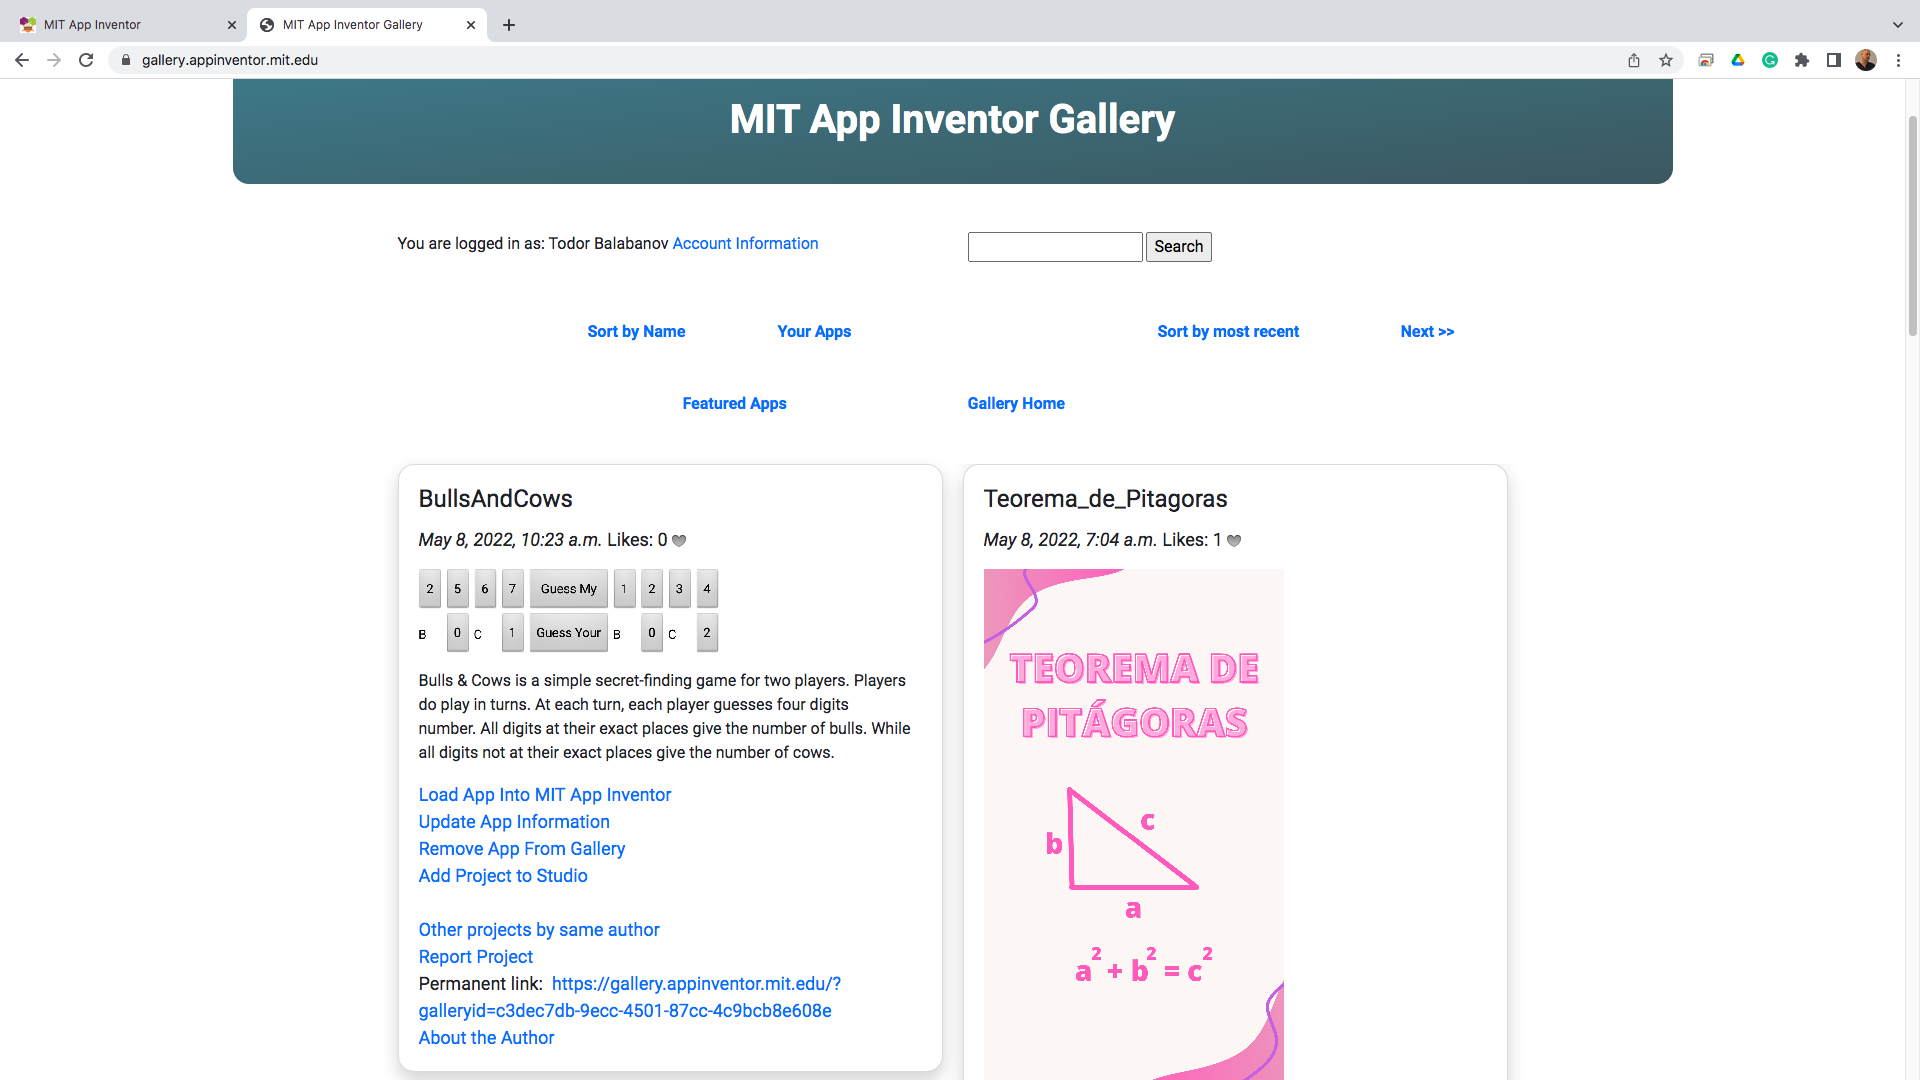
\includegraphics[width=1.0\linewidth,height=0.5\linewidth]{fig080031.png}
  \caption{Страница на публикувания проект}
\label{fig080031}
\end{figure}

Макар и пълнофункционална, играта все още не е завършена до нивото на краен продукт. Липсват серия от проверки за това дали потребителят въвежда коректно числата (примерно повтарящи се цифри). Липсва функционалност за обявяване на победителя, въпреки че появата на четири бика ясно обозначават кой побеждава. Липсва екран с помощна информация, както и звуково оформление. Липсващата функционалност е извън обхвата на настоящото изложение и би могла да послужи, като допълнително упражнение за желаещите да надградят знанията си.

